\documentclass[11pt]{article}

\usepackage{amsmath}
\usepackage{amsfonts}
\usepackage{amssymb}
\usepackage{amsthm}
\usepackage{graphicx}
\usepackage{subcaption}
\usepackage[colorinlistoftodos]{todonotes}
\usepackage[colorlinks=true, allcolors=blue]{hyperref}
\usepackage{showlabels}
\usepackage{palatino}
\usepackage{hyphenat}
\usepackage{thm-restate}
\usepackage{natbib}
\usepackage{setspace}
\onehalfspacing
\usepackage{authblk}

% Line numbers and some weirdness
\usepackage{lineno}
\linenumbers
\newcommand*\patchAmsMathEnvironmentForLineno[1]{%
  \expandafter\let\csname old#1\expandafter\endcsname\csname #1\endcsname
  \expandafter\let\csname oldend#1\expandafter\endcsname\csname end#1\endcsname
  \renewenvironment{#1}%
     {\linenomath\csname old#1\endcsname}%
     {\csname oldend#1\endcsname\endlinenomath}}% 
\newcommand*\patchBothAmsMathEnvironmentsForLineno[1]{%
  \patchAmsMathEnvironmentForLineno{#1}%
  \patchAmsMathEnvironmentForLineno{#1*}}%
\AtBeginDocument{%
\patchBothAmsMathEnvironmentsForLineno{equation}%
\patchBothAmsMathEnvironmentsForLineno{align}%
\patchBothAmsMathEnvironmentsForLineno{flalign}%
\patchBothAmsMathEnvironmentsForLineno{alignat}%
\patchBothAmsMathEnvironmentsForLineno{gather}%
\patchBothAmsMathEnvironmentsForLineno{multline}%
}

% commented for arXiv submission
%\usepackage{fancyhdr}
% \fancyhead[R]{ submission intended as Article in Discoveries section of \emph{MBE} }


\graphicspath{ {figures/} }

% http://bytesizebio.net/2013/03/11/adding-supplementary-tables-and-figures-in-latex/
\newcommand{\beginsupplement}{%
        \setcounter{table}{0}
        \renewcommand{\thetable}{S\arabic{table}}%
        \setcounter{figure}{0}
        \renewcommand{\thefigure}{S\arabic{figure}}%
     }

% Commands
\newtheorem{theorem}{Theorem}
\newtheorem{lemma}[theorem]{Lemma}
\newtheorem*{definition}{Definition}

\newcommand{\alphabet}{\mathcal{A}}
\newcommand{\fullAlignment}{\mathbf{Y}}
\newcommand{\alignmentColumn}{\mathbf{y}}
\newcommand{\alignmentColumnRV}{Y}
\newcommand{\siteSplit}{\tilde{y}}
\newcommand{\siteSplitSet}{\mathcal{Y}}
\newcommand{\fullAncestralStates}{\mathbf{H}}
\newcommand{\ancestralStateColumn}{\mathbf{h}}
\newcommand{\ancestralStateColumnRV}{H}
\newcommand{\ancestralSplit}{\tilde{h}}
\newcommand{\ancestralSplitSet}{\mathcal{H}}
\newcommand{\ancestralSplitPartition}{\eta}
\newcommand{\fullAncestralSplitPartitions}{\boldsymbol\eta}

\newcommand{\patternToSplit}{\psi}
\newcommand{\ancestralToSplit}{\xi}

\newcommand{\siteSplitRV}{\Psi}
\newcommand{\ancestralSplitRV}{\Xi}

\newcommand{\nCols}{n}
\newcommand{\nSiteRows}{m}
\newcommand{\nAncestralStateRows}{p}
\newcommand{\nSiteSplits}{q}
\newcommand{\nAncestralSplits}{r}

\newcommand{\shannonDivergence}{D}

\DeclareMathOperator*{\argmax}{argmax}

\allowdisplaybreaks

\title{Joint maximum-likelihood of phylogenies and ancestral states is not consistent}

\author[1]{David A. Shaw}
\author[1]{Frederick A. Matsen IV\thanks{Corresponding author. Email: \url{matsen@fredhutch.org}}}
\affil[1]{Computational Biology Program, Fred Hutchinson Cancer Research Center\\ Seattle, WA, USA}
\date{}

\begin{document}

\renewcommand{\arraystretch}{1.2} % because otherwise exponents get eaten by \hline

\maketitle
% commented for arXiv submission
%\thispagestyle{fancy}

\begin{abstract}
Maximum likelihood estimation in phylogenetics requires a means of handling unknown ancestral states.
Classical maximum likelihood averages over these unknown intermediate states, leading to consistent estimation of the topology and continuous model parameters.
Recently, a computationally-efficient approach was proposed to jointly maximize over these unknown states and phylogenetic parameters.
Although this method of joint maximum likelihood estimation can obtain estimates more quickly, its properties as an estimator are not yet clear.
In this paper, we show that this method of jointly estimating phylogenetic parameters along with ancestral states is not consistent in general.
We find a set of parameters that generate data under a four-taxon tree for which this joint method estimates an incorrect topology in the limit of infinite-length sequences.
For branch length estimation on the correct topology, we outline similar cases where branch length estimates are consistently and heavily biased.
\end{abstract}

\newpage

\section*{Introduction}

Classical maximum likelihood (ML) estimation in phylogenetics operates by integrating out latent ancestral states at the internal nodes of the tree.
In a recent paper, \citet{Sagulenko2017-jo} suggest using an approximation to ML inference in which the likelihood is maximized jointly across model parameters and ancestral sequences on a fixed topology.
This is attractive from a computational perspective: such joint inference can proceed according to an iterative procedure in which ancestral sequences are first estimated and model parameters are optimized conditional on these estimates.
This latter conditional optimization is simpler and more computationally efficient than optimizing the marginal likelihood.
But is it statistically consistent?

An estimator is said to be statistically consistent if it converges to the generating model with probability 1 in the large-data limit; existing consistency proofs for maximum likelihood phylogenetics \citep{RoyChoudhury2015-ta} apply only to estimating model parameters when the ancestral sequences have been integrated out of the likelihood.
These proofs do not readily extend to include estimating ancestral states.
Moreover, examples of inconsistency arising from problems where the number of parameters increases with the amount of data \citep{Neyman1948-tt} indicate that joint inference of trees and ancestral states may not enjoy good statistical properties.
In this case those additional parameters come in the form of the states of ancestral sequences.
%page 2 section 2.1 at the top of the second column first paragraph second sentence
Although the software described in \citet{Sagulenko2017-jo} fits on a user-supplied topology and the authors explicitly warn that the approximation is for the case where ``branch lengths are short and only a minority of sites change on a given branch,'' their work motivates understanding the general properties of such joint inference.
In particular, one would like to know when this approximate technique breaks down for both topology and branch length inference, even when sequence data is ``perfect,'' i.e., is generated without sampling error according to the exact model used for inference.

In this paper, we show that the joint inference of trees and ancestral sequences is not consistent in general.
To do so, we use a binary symmetric model with data being generated on the four-taxon ``inverse Felsenstein (InvFels)'' tree---also called the ``Farris'' tree \citep{Siddall1998-hq, Felsenstein2004}---and we construct bounds on the joint objective function to demarcate a sizeable area of long branch lengths in which joint inference is guaranteed to give the wrong tree in the case of perfect sequence data with an infinite number of sites.
We find similar areas where joint inference consistently overestimates interior branch lengths when the topology is known and fixed.

\section*{Phylogenetic maximum likelihood}

Assume the binary symmetric model, namely with a character alphabet $\alphabet=\{0,1\}$ and a uniform stationary distribution \citep{Semple2003-em}.
Let $\nSiteRows$ be the number of tips of the tree, and $\nAncestralStateRows = \nSiteRows-2$ the number of internal nodes.
We observe $\nCols$ independent and identically distributed samples of character data, i.e., an alignment with $\nCols$ columns, $\fullAlignment=[\alignmentColumn_1,\ldots,\alignmentColumn_\nCols]\in\alphabet^{\nSiteRows\times\nCols}$ distributed as the random variable $\alignmentColumnRV$.
The corresponding unobserved ancestral states are $\fullAncestralStates=[\ancestralStateColumn_1,\ldots,\ancestralStateColumn_\nCols]\in\alphabet^{\nAncestralStateRows\times\nCols}$ and distributed as $\ancestralStateColumnRV$ with each $\ancestralStateColumn_i\in\alphabet^\nAncestralStateRows$.

We parameterize branches on the unique unrooted four-tip phylogenetic tree in ways known as the ``InvFels'' and ``Felsenstein'' trees (Fig.~\ref{fig:farris-fels-top}).
In the standard configuration of each of these trees, the interior branch length parameters are equal to the bottom two parameters.
We show in the Appendix that, in the case of the InvFels tree, performing inference fixing both the top two branch parameters to be equal and the bottom two branch parameters to be equal will obtain the same maximum likelihood estimate as in the case of arbitrary branch parameters.

\begin{figure}
\centering
\begin{subfigure}{.45\linewidth}
\centering
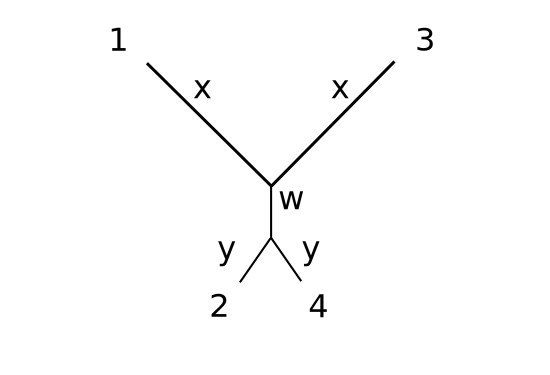
\includegraphics[width=\textwidth]{farris_blank}
\caption[short]{InvFels tree $\tau_1$}
\end{subfigure}
\begin{subfigure}{.45\linewidth}
\centering
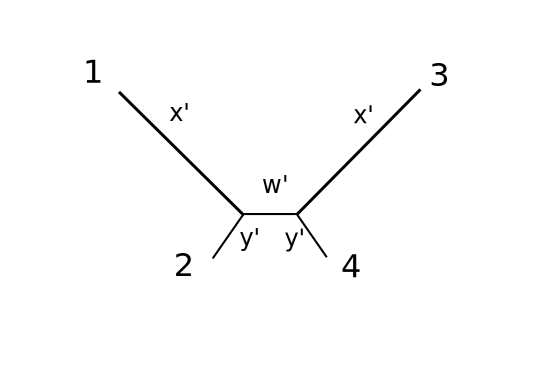
\includegraphics[width=\textwidth]{felsenstein_blank}
\caption[short]{Felsenstein tree $\tau_2$}
\end{subfigure}
\caption{Two four-taxon trees with fidelities as labeled: $\theta_1=\theta_3=x$, $\theta_2=\theta_4=y$, and $\theta_5=w$.
}
\label{fig:farris-fels-top}
\end{figure}

We parameterize the branches of these trees not with the standard notion of branch length in terms of number of substitutions per site, but with an alternate formulation called ``fidelity.''
The probability of a substitution on a branch with fidelity $\theta$ is $(1-\theta)/2$ while the probability of no substitution is $(1+\theta)/2$ where $0 \le \theta \le 1$.
This parameter quantifies the fidelity of transmission of the ancestral state across an edge \citep{Matsen2007-jq}.

Fidelities have useful algebraic properties.
As data becomes plentiful, we use the Hadamard transform (see \eqref{eq:hadamard_probability} in the Appendix) to compute the exact probabilities that generate each particular configuration of taxa---we call these ``generating probabilities''---and these have an especially simple form.
For a four-taxon tree, define the general branch fidelity parameter $t=\{\theta_1,\theta_2,\theta_3,\theta_4,\theta_5\}$ where fidelities are ordered in the order of the taxa with the internal branch last (Fig.~\ref{fig:farris-fels-top}).
We show in the Appendix that, for the InvFels tree, the maximum likelihood fidelities require $\theta_1=\theta_3$ and $\theta_2=\theta_4$, so we subsequently fix fidelity parameters to $t=\{x,y,x,y,w\}$.

\subsection*{Two paths to maximum likelihood}

The standard phylogenetic likelihood approach on unrooted trees under the usual assumption of independence between sites is as follows.
For a topology $\tau$ and branch fidelities $t$ the likelihood given observed ancestral states $\fullAncestralStates$ is
\begin{equation}
\label{eq:full_likelihood}
L_\nCols(\tau, t; \fullAlignment,\fullAncestralStates) = \prod_{i=1}^{\nCols} \ \Pr(\alignmentColumnRV=\alignmentColumn_i, \ancestralStateColumnRV=\ancestralStateColumn_i \mid \tau, t).
\end{equation}
The probability $\Pr(\alignmentColumnRV=\alignmentColumn_i, \ancestralStateColumnRV=\ancestralStateColumn_i \mid \tau, t)$ is a product of transition probabilities determined by $\fullAlignment$, $\fullAncestralStates$, $\tau$, and $t$ \citep{Felsenstein2004}.

The classical approach is to maximize the likelihood marginalized across ancestral states
\begin{equation}
\label{eq:marginal_likelihood}
\tilde{L}_\nCols(\tau, t; \fullAlignment) = \prod_{i=1}^{\nCols} \ \sum_{\ancestralStateColumn_i\in\alphabet^{\nAncestralStateRows}} \ \Pr(\alignmentColumnRV=\alignmentColumn_i, \ancestralStateColumnRV=\ancestralStateColumn_i \mid \tau, t)
\end{equation}
to estimate the tree $\tau$ and branch fidelities $t$.

The alternative approach \citep{Sagulenko2017-jo} does away with the marginalization and directly estimates the maximum likelihood parameters of the fully-observed likelihood in \eqref{eq:full_likelihood}.
This is known in statistics as a profile likelihood \citep{Murphy2000-ry}, which exists here because $\alphabet$ is a finite set:
\begin{equation}
\label{eq:profile_likelihood}
L_\nCols'(\tau, t; \fullAlignment) = \prod_{i=1}^{\nCols} \ \max_{\ancestralStateColumn_i\in\alphabet^{\nAncestralStateRows}} \ \Pr(\alignmentColumnRV=\alignmentColumn_i, \ancestralStateColumnRV=\ancestralStateColumn_i \mid \tau, t) = \max_{\fullAncestralStates\in\alphabet^{\nAncestralStateRows\times\nCols}} \ L_\nCols(\tau, t; \fullAlignment, \fullAncestralStates).
\end{equation}
We use $\hat{\fullAncestralStates}$ to denote an estimate for $\fullAncestralStates$ obtained by maximizing \eqref{eq:profile_likelihood}, and estimate a topology and branch fidelities using this profile likelihood as
\begin{equation}
\label{eq:profile_likelihood_topology_bl}
(\hat{\tau}, \hat{t}) = \argmax_{\tau, t} \ L_\nCols'(\tau, t; \fullAlignment).
\end{equation}
In general, the functional form of \eqref{eq:profile_likelihood} is determined by inequalities arising from taking maxima row-wise in Tables~\ref{tab:farris_likelihoods} and~\ref{tab:fels_likelihoods} to obtain the likelihood term for each most likely ancestral state, these terms depending on the unknown $(\tau, t)$.
For this reason, in practice, the joint inference strategy estimates $\hat{\fullAncestralStates}$ for a fixed $(\tau,t)$, then $(\hat{\tau},\hat{t})$ given $\hat{\fullAncestralStates}$, maximizing each of these conditional objectives until convergence \citep{Sagulenko2017-jo}.


\section*{Inconsistency of joint inference}

We now state our results on the inconsistency of joint inference.
All proofs are deferred to the Appendix.

Assume $\fullAlignment$ is generated from topology $\tau^*$ and branch fidelities $t^*$.
Use $\ell_{\tau^*,t^*}(\tau, t)$ to denote the expected per-site log-likelihood, which can be thought of as the infinite-length sequence case
\[
\frac{1}{n}\log L_\nCols'(\tau, t; \fullAlignment) \rightarrow \ell_{\tau^*,t^*}(\tau, t).
\]
We give $\ell$ explicitly as \eqref{eq:site_pattern_profile_likelihood_mean} in the Appendix.

\subsection*{Inconsistency in topology estimation}

To show an inconsistency in topology estimation, we start with true generating parameters $t^*=\{x^*, y^*, x^*, y^*, y^*\}$ on the InvFels topology (Fig.~\ref{fig:farris-fels-top}a).
We show that, as $\nCols\rightarrow\infty$, there exist values for $x^*$ and $y^*$ such that the value of the likelihood after maximizing using joint inference is greater for the Felsenstein topology ($\tau_2$) than for the true, generating InvFels topology ($\tau_1$).
To do so, we construct an upper bound $C_0(x^*, y^*)$ for the likelihood given the InvFels topology as a function of $x^*$ and $y^*$ and, similarly, a lower bound $C_1(x^*, y^*)$ for the likelihood given the Felsenstein topology.
When $C_0(x^*, y^*) < C_1(x^*, y^*)$, the likelihood in the Felsenstein case is larger than the likelihood in the InvFels case, demonstrating inconsistency (Fig.~\ref{fig:inconsistency-farris}).
\begin{restatable}{theorem}{topoInconsist}
Let $t^*=\{x^*, y^*, x^*, y^*, y^*\}$ and $t=\{x, y, x, y, w\}$.
There exist $C_0(x^*, y^*), C_1(x^*, y^*),$ and a set of $0 < x^*, y^* < 1$ such that
\[
\max_{t} \ \ell_{\tau_1,t^*}(\tau_1, t) \le C_0(x^*, y^*),
\]
\[
C_1(x^*, y^*) \le \max_{t} \ \ell_{\tau_1,t^*}(\tau_2, t)
\]
with $C_0(x^*, y^*) < C_1(x^*, y^*)$.
\end{restatable}
The proof of this theorem is by a detailed examination of inequalities.
Intuitively, $\tau_2$ is favored in performing joint inference since the objective function for $\tau_2$ has more ``degrees of freedom''---Table~\ref{tab:likelihoods} shows that $\tau_1$ has only three possible forms for its objective function while $\tau_2$ has many more.
This enables more possible maxima for $\tau_2$ even if data are generated from $\tau_1$.

\begin{figure}
\centering
% obtained by running
% python joint_inf_plot.py --analytic --topology --delta .001 --plot-name figures/topology-inconsistency.svg
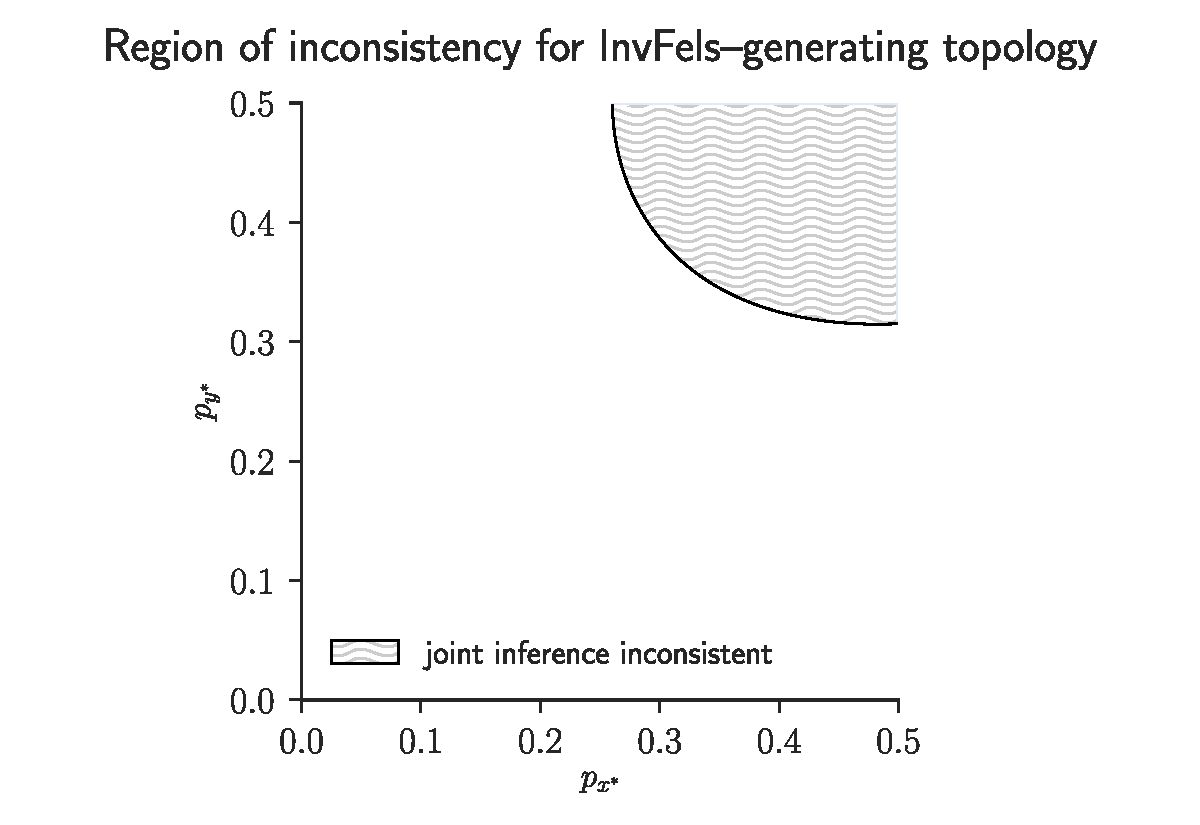
\includegraphics[width=\textwidth]{topology-inconsistency-inkscape}
\caption{
    An analytically-derived region of topological inconsistency in terms of fidelities for ``perfect'' data generated on the InvFels topology (Fig.~\ref{fig:farris-fels-top}) with $w^* = y^*$.
    Due to the looseness of the upper and lower bounds, the parameters in the white region do not necessarily indicate consistency, though all parameters in the shaded region result in an inconsistency.
}
\label{fig:inconsistency-farris}
\end{figure}

\subsection*{Inconsistency in branch length estimation}

%EM Line numbering has a huge gap here. Could you look around and see if you see anything about this on the web?
%das: fixed
We now consider the problem of branch length estimation on the correct tree using joint estimation.
As described above, we use the notion of fidelities to analyze what happens as changes occur along each branch as opposed to the standard branch length formulation.
We analyze two settings on the InvFels tree, corresponding to whether some branch fidelities are fixed at their true values or not.
As above, assume that data is generated from the InvFels tree with two top branches of fidelity $x^*$ and all other branches of fidelity $y^*$ (Fig.~\ref{fig:farris-fels-top}).
In the first ``restricted'' case, we show that for a nontrivial subset of possible values for $x^*$ and $y^*$, the interior branch fidelity parameter $w$ will be consistently overestimated as exactly equal to one (zero branch length) instead of its true value of $y^*$.
That is, if we estimate $x$ and $y$ correctly, then, for
\[
\hat{w} = \arg\max_{w} \ \ell_{\tau_1,t^*}(\tau_1, \{x^*,y^*,x^*,y^*,w\}),
\]
there is a set of values for $x^*$ and $y^*$ where $\hat{w}\equiv 1$.
In the general case, we do the same but with
\[
(\hat{x}, \hat{y}, \hat{w}) = \arg\max_{x,y,w} \ \ell_{\tau_1,t^*}(\tau_1, \{x,y,x,y,w\})
\]
to find a region where the inferred values do not converge to the generating values.
These situations are in contrast to the approach using marginal likelihood where $\hat{w}$ necessarily converges to $y^*$ as the number of observations grows \citep{RoyChoudhury2015-ta}.

\subsubsection*{Restricted case}

Fix estimated fidelities $x=x^*$ and $y=y^*$ to their true, generating values and estimate the internal branch parameter $w$.
\begin{restatable}{theorem}{restrictedBranchInconsist}
\label{thm:restricted-bl}
Let
\[
\beta := \beta(x^*, y^*) = 1+(x^*)^2+(y^*)^2+(x^*)^2(y^*)^2,
\]
\[
\gamma := \gamma(x^*, y^*) = 4x^*y^*.
\]
The maximum likelihood value $\hat{w}$ is equal to 1 if
\[
%\beta^2-\gamma^2-2\gamma^2\alpha_1-2\gamma^2\alpha_2+2\gamma\alpha_1\beta-2\gamma\alpha_2\beta \ge 0.
-\gamma^2\left(1 + \frac{1}{2}\beta\right) + 2\gamma\beta x^*(y^*)^2 + \beta^2 \ge 0
\]
and there exists a set of $0 < x^*, y^* < 1$ satisfying this.
\end{restatable}
This theorem allows us to demarcate a region of biased internal branch length estimation by plotting where the inequality in Theorem~\ref{thm:restricted-bl} is satisfied (Fig.~\ref{fig:bl-inconsistency}).
Intuitively, this happens when estimated ancestral sequences at internal nodes are identical across a branch with this branch length estimated to be zero (i.e., has fidelity $\hat{w} = 1$).
We provide the following as an intuition for the theoretical development.
For a particular site pattern, in obtaining the joint maximum likelihood function we maximize over ancestral states.
For the internal branch---the branch between the two internal nodes---we have a choice of $(1+w)$ or $(1-w)$ in each of our likelihood terms depending on which ancestral state split corresponds to the highest partial likelihood term.
A maximization procedure will more likely introduce a $(1+w)$ term than a $(1-w)$ term, though this will not be guaranteed as the maximum depends on the values of $x$ and $y$.
This tendency to more likley include $(1+w)$ terms in the likelihood results in a positive bias of branch fidelities.
If we allow multifurcating trees in our inference, then we can think of this as another instance of converging to the wrong topology.

\begin{figure}
\centering
% obtained by running
% python joint_inf_plot.py --analytic --restricted-branch-lengths --delta .001 --plot-name figures/branch-length-inconsistency.svg
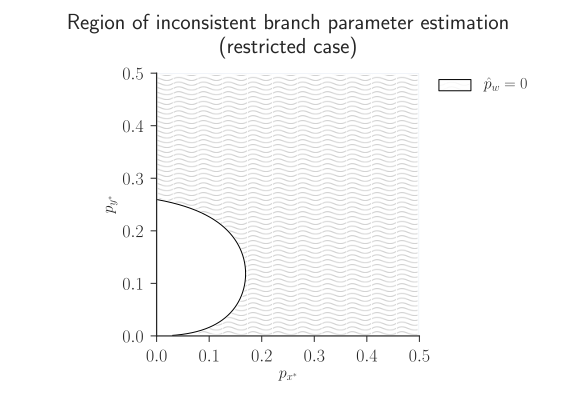
\includegraphics[width=\textwidth]{branch-length-inconsistency-inkscape}
\caption{Analytically-derived region of branch parameter inconsistency in terms of fidelities $x=x^*$ and $y=y^*$ that are fixed to their correct values with the same data-generating setup as Fig.~\ref{fig:inconsistency-farris}.
The shaded region shows the area in which the internal branch length is estimated to be 0, i.e.\ the estimated fidelity $\hat{w} = 1$, even though the generating fidelity is $y^*$.
Here again, the shaded region is guaranteed to give inconsistent estimation, while the white region may or may not do so.}
\label{fig:bl-inconsistency}
\end{figure}

\subsubsection*{General case}

The general case is more challenging to analyze and so we obtain weaker bounds.
Here, $\hat{w}$ is a function of $x^*$, $y^*$, $\hat{x}$, and $\hat{y}$.
Looking to the previous section, the region where $\hat{w}=1$ will still be given by the inequality in Theorem~\ref{thm:restricted-bl}, only with $\gamma$ and $\beta$ now being functions of $\hat{x}$ and $\hat{y}$ instead of $x^*$ and $y^*$.
Assume we know $\hat{x}$ and $\hat{y}$ as functions of $x^*$ and $y^*$.
We show there are similar bounds as in the restricted case, though we need to take into account the unknown values of $\hat{x}$ and $\hat{y}$.
We fix bounds on these estimates and show that, in the general case, joint estimation either estimates $\hat{w}$ to be one or estimates $\hat{x}$ or $\hat{y}$ to fall outside of specified bounds, indicating a poor estimate in at least one of the three unknown branch parameters.
\begin{restatable}{theorem}{generalBranchInconsist}
\label{thm:general-bl}
Define $\gamma(x, y) = 4xy$.
For
\[
\beta := \beta(x^*, y^*) = 1+(x^*)^2+(y^*)^2+(x^*)^2(y^*)^2,
\]
\[
\gamma := \gamma(x^*, y^*),
\]
bounds
\[
\gamma_L := \gamma_{L}(x^*, y^*) \le \gamma(\hat{x}, \hat{y}),
\]
\[
\gamma_U := \gamma_{U}(x^*, y^*) \ge \gamma(\hat{x}, \hat{y}),
\]
and
\[
\beta_L := \beta_{L}(x^*, y^*) \le \beta(\hat{x}, \hat{y}),
\]
the maximum likelihood value $\hat{w}=1$ when
\[
-\gamma_{U}^2\left(1 + \frac{1}{2}\beta\right) + 2\gamma_{L}\beta_{L}x^*(y^*)^2 + \beta_{L}^2 \ge 0.
\]
\end{restatable}
We use this theorem to show incorrect branch parameter estimates as follows.
If we do not tolerate any error in pendant branches, we use the tightest possible bounds $\gamma_{L} = \gamma_{U} = \gamma$ and $\beta_{L} = \beta$, which is the restricted case of the previous section (Fig.~\ref{fig:bl-inconsistency}).
For an intermediate bound, define a specified allowable level of error in estimates for $\hat{x}$ and $\hat{y}$ so that
\[
x^*-x_{L} \le \hat{x} \le x^*+x_{U}
\]
and
\[
y^*-y_{L} \le \hat{y} \le y^*+y_{U}.
\]
Then $\gamma_L, \gamma_U$ and $\beta_L$ can be derived directly from the bounds on $\hat{x}$ and $\hat{y}$.
As an example, the region to the left side of the curve in Fig.~\ref{fig:bl-loose-inconsistency} shows the case where $x_L=x_U=y_L=y_U=0.1$.
In this case, joint inference will either estimate $\hat{w}$ to have fidelity one or estimate either $\hat{x}$ or $\hat{y}$ to be more than $0.1$ away from its true fidelity.

\begin{figure}
\centering
% obtained by running
% python joint_inf_plot.py --analytic --general-branch-lengths --delta .001 --plot-name figures/bl-loose-inconsistency.svg
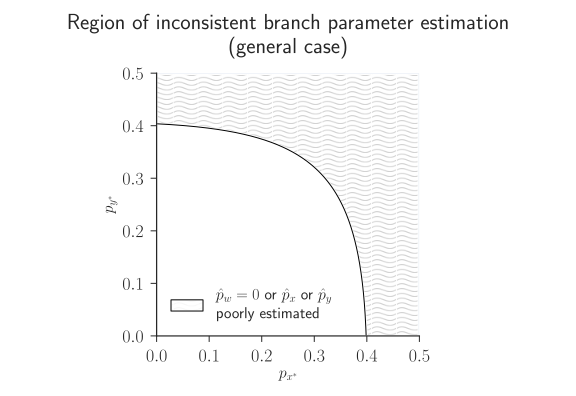
\includegraphics[width=\textwidth]{bl-loose-inconsistency-inkscape}
\caption{
    Analytically-derived region of branch parameter inconsistency in terms of fidelities with the same data-generating setup as Fig.~\ref{fig:inconsistency-farris}.
    In the marked region, either $\hat{w}=1$ or one of $x^*-0.1 \le \hat{x} \le x^*+0.1$ or $y^*-0.1 \le \hat{y} \le y^*+0.1$ will not be true, resulting in poor estimation of the pendant branch parameters.
    As in previous plots, the shaded and white regions are loose indications of inconsistency.
}
\label{fig:bl-loose-inconsistency}
\end{figure}

\subsubsection*{Empirical validation}

Direct numerical optimization confirms our theoretically-derived bounds and provides a more detailed picture compared to the conservative analytically-derived region (Fig.~\ref{fig:bl-loose-inconsistency}).
To determine how conservative, we use the method of basin-hopping \citep{Wales1997} to perform joint estimation (Fig.~\ref{fig:bl-general-inconsistency}).
We see that the region of inconsistency in the general case is similar to that of the restricted case (compare Figs.~\ref{fig:bl-inconsistency} and~\ref{fig:bl-general-inconsistency}).
This region encompasses the majority of the branch fidelity space; even given the correct topology and performing our best possible optimization, we have many situations where we will estimate the interior branch fidelity to be one.

We provide a full description of our optimization procedure in the Appendix, but briefly, we perform two maximizations---one over $0 \le x,y,w \le 1$ and one over $0 \le x,y \le 1$ with $w=1$---and take the value of $\hat{w}$ with the higher objective function.
We compute these maxima over a lattice in steps of $10^{-2}$ for $x^*$ and $y^*$ from $10^{-2}$ to $1-10^{-2}$.
We do not include zero or one in our lattice to further stabilize the fits, as these cases can result in pathologies.
Our optimization code can be found at \url{https://github.com/matsengrp/joint-inf/}.

As data were generated with parameters $\{x^*, y^*, x^*, y^*, y^*\}$, the true value for $w$ is $y^*$.
Marginal inference performs as expected, where $\hat{w}$ is equal to $y^*$ regardless of the value of $x^*$ (Fig.~\ref{fig:bl-general-marginal}) when optimizing \eqref{eq:marginal_likelihood} using the same procedure.
For joint inference, the estimates for $\hat{w}$ when $x^*$ and $y^*$ are both large look reasonable, with $\hat{w}$ increasing as $y^*$ increases, though Fig.~\ref{fig:bl-general-bias} shows there is a systematic positive bias in this procedure even when $\hat{w}$ is not estimated to be one.
To understand the quality of each fit, we report the range of $\hat{w}-y^*$ where $\hat{w}\neq 1$.
For joint inference, the errors range from $[-7\times 10^{-3}, 8\times 10^{-2}]$ and for marginal inference, $[-8\times 10^{-8}, 5\times 10^{-7}]$ showing that, even in cases where joint inference does not estimate $\hat{w}$ to be exactly one, it still fails to achieve a low error from truth.

\begin{figure}
\centering
% obtained by running
% python joint_inf_plot.py --empirical --general-branch-lengths --delta .01 --plot-name figures/w-hat-empirical-01.svg --out-pkl-name figures/w-hat-empirical-01.pkl --n-jobs 16
% or
% python joint_inf_plot.py --empirical --general-branch-lengths --plot-name figures/w-hat-empirical-01.svg --in-pkl-name figures/w-hat-empirical-01.pkl
% if fit already
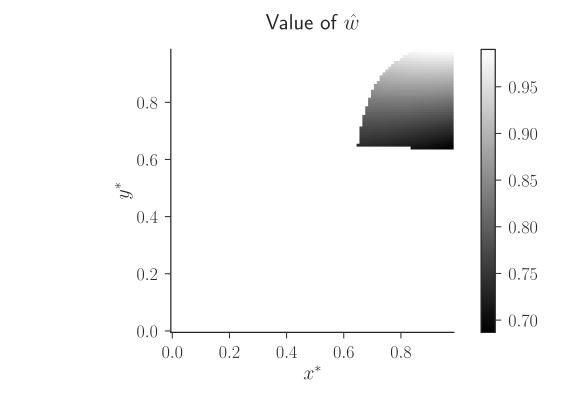
\includegraphics[width=\textwidth]{w-hat-empirical-01}
\caption{
    Numerical estimates for $\hat{w}$ when computing $(\hat{x}, \hat{y}, \hat{w})$ using basin-hopping \citep{Wales1997} optimizing \eqref{eq:profile_likelihood}.
    Data generated as in Fig.~\ref{fig:inconsistency-farris}.
}
\label{fig:bl-general-inconsistency}
\end{figure}

\section*{Discussion}

We have shown that jointly inferring ancestral states and phylogenetic parameters \citep{Sagulenko2017-jo} is not consistent in general.
Specifically, in the case of four-taxon trees with infinite data, we have obtained nontrivial regions of generating parameters that result in two types of inconsistency: first, where joint inference converges on the incorrect topology and, second, where it estimates severely biased branch lengths even given the correct topology.
In all cases, these regions of inconsistency arise when the branches of the generating trees are ``long,'' that is, when branch fidelities tend to be small.
This inconsistency in the case of long branches concurs with some empirical findings in \citet{Sagulenko2017-jo}, namely their Figures~2 and 3.

Joint inference of tree parameters and ancestral sequences is a type of profile likelihood, a well-studied subject in statistics \citep{Murphy2000-ry}.
Many properties regarding the performance of maximum likelihood estimates obtained using this approach are known, and many methods exist to overcome their undesirable properties, e.g., the method of sieves \citep{Geman1982}.
A potential solution in this case using the method of sieves could be to project the column-wise ancestral state patterns into a lower-dimensional space, allowing the degrees of freedom in the ancestral state columns to grow with $\nCols$, albeit more slowly than $O(\nCols)$.
Elsewhere in statistics literature, the failure of maximum likelihood estimates to obtain consistent estimates as the number of parameters goes to infinity have been shown by the Neyman-Scott paradox \citep{Neyman1948-tt}, though parameters tending to infinity is not a necessary condition for inconsistency \citep{LeCam1990}.
Consistency proofs of standard maximum likelihood estimates of phylogeny \eqref{eq:marginal_likelihood} are recent \citep{RoyChoudhury2015-ta}, and no results have been obtained for profile likelihood.
We have furthered progress in understanding the limitations of this joint optimization procedure.

Previous work in phylogenetics has developed consistency counterexamples using the same four-taxon topologies used here \citep{Felsenstein1978-rr}.
In this previous work, when simulating data under the Felsenstein topology $\tau_2$, as the number of observations increases, the InvFels topology $\tau_1$ becomes more likely when performing a particular estimation procedure.
This is the converse of what we have shown for joint inference, where the Felsenstein topology is more likely than the InvFels topology.
Moreover, the inconsistency demonstrated by \citet{Felsenstein1978-rr} is attributed to long branch attraction, i.e., the fact that there may be multiple long branches where parallel changes are more likely than a single change along a short branch.
This is not the case here; for our case, the inconsistency generally occurs when all branches are long, and has more to do with the choices of the form of the likelihood than from the interplay of long and short branches.
Difficulties in phylogenetic estimation when generating data on the InvFels tree have been found by \citet{Siddall1998-hq}, though \citet{Swofford2001-hr} show that sequence length plays a major role in these issues.

While we have shown inconsistency in both topology and branch parameter estimation, there is substantial scope for future work to make these results more precise and more general.
The techniques used to obtain upper and lower bounds for the likelihoods in the topology estimation case provide relatively loose bounds, though how loose they are remain unknown without either further analysis or verification through simulation.
Similarly, for the general case in estimating branch lengths, we were only able to provide a conservative region of overestimation, and the unusual shape we observe via numerical optimization (Fig.~\ref{fig:bl-general-inconsistency}) begs further investigation.
Empirical validation shows that the general case is not unlike the restricted case.
All of these results hold only for a simple binary symmetric model on four-taxon trees, and extensive simulation is necessary to understand how these results extend to more complicated general cases.
Given that many of the bounds presented here are in the form of level sets of multivariate polynomials, a more formal approach using algebraic geometric techniques may reveal more stable or interesting patterns of inconsistency; see \citet{Sturmfels2002} for a thorough treatment of solving systems of polynomial equations.
Finally, all of the material presented here concerns joint estimation under maximum likelihood, and does not pose any problem for other settings, such as joint sampling of trees and ancestral sequences in a Bayesian framework.


\section*{Acknowledgements}
We thank Richard Neher, Vladimir Minin, and Joe Felsenstein for helpful discussions.

This work was supported by National Institutes of Health grants R01-GM113246, R01-AI120961, U19-AI117891, and U54-GM111274 as well as National Science Foundation grants CISE-1561334 and CISE-1564137.
The research of Frederick Matsen was supported in part by a Faculty Scholar grant from the Howard Hughes Medical Institute and the Simons Foundation.

\bibliographystyle{plainnat}
\bibliography{joint_inf}

\newpage
\beginsupplement

\section*{Appendix}

\subsection*{Site split formulation}
We begin by introducing ``site splits,'' which formalize the notion that a given site pattern is equally probable to its complement under the binary symmetric model.
This is a standard step in the description of the Hadamard transform (Section 8.6 of \citet{Semple2003-em}), although our approach is complicated slightly by the inclusion of ancestral states.

Since we have a finite character alphabet, for a given column $i$ there are a finite number of possible assignments of characters to tips $\alignmentColumn_i$ or internal nodes $\ancestralStateColumn_i$; this results in a simplification of likelihood calculation.
Take the tip labels of $\tau$ to be $\{1,\ldots,\nSiteRows\}$.
For likelihood calculation under the binary symmetric model, we describe a given $\alignmentColumn_i$ as a subset of indices $\siteSplit\subseteq\siteSplitSet:=\{1,\ldots,\nSiteRows-1\}$ with equivalent characters, commonly called a ``site split.''
We define the site split $\siteSplit$ for a $\alignmentColumn_i$ as simply $\alignmentColumn_i$ if the label $\nSiteRows$ is not in $\alignmentColumn_i$, and as its complement otherwise.
Taking such a complement simplifies but does not change the result of likelihood computation because the probability of observing a particular collection of binary characters is equivalent to the probability of its complement under the binary symmetric model.

For topology $\tau$, we define an ordered set of internal node labels $\{1,\ldots,\nAncestralStateRows\}$ for $\ancestralStateColumn_i$ and similarly use a subset of characters $\ancestralSplit\subseteq\ancestralSplitSet:=\{1,\ldots,\nAncestralStateRows\}$ to describe a realization $\ancestralStateColumn_i$.
In this case the entire set of internal nodes must be enumerated: the probability of observing an ancestral state split conditional on a site split is not invariant to taking its complement.

We enumerate the site splits $\siteSplit_j$ of which there are $\nSiteSplits=|\mathcal{P}(\siteSplitSet)|$ in total where $\mathcal{P}$ denotes the power set.
Similarly we enumerate ancestral splits $\ancestralSplit_k$ of which there are $\nAncestralSplits=|\mathcal{P}(\ancestralSplitSet)|$ in total.

We first fix notation.
\begin{definition}
Let the mapping from site patterns to site splits be
$$
\patternToSplit:\alphabet^\nSiteRows\rightarrow\mathcal{P}(\siteSplitSet)
$$
and the mapping from ancestral states and tip states to ancestral state splits be
$$
\ancestralToSplit:\alphabet^\nAncestralStateRows\times\alphabet^\nSiteRows\rightarrow\mathcal{P}(\ancestralSplitSet).
$$
Then, given a site pattern--valued random variable $\alignmentColumnRV$, define the random variable
$$
\siteSplitRV := \patternToSplit(\alignmentColumnRV)
$$
that takes corresponding realizations $\siteSplit_j$ for some $j$, and
$$
\ancestralSplitRV := \ancestralToSplit(\alignmentColumnRV, \ancestralStateColumnRV)
$$
for a tip state--valued random variable $\alignmentColumnRV$ and an ancestral state--valued random variable $\ancestralStateColumnRV$.
\end{definition}
The mapping $\patternToSplit$ takes the complement of site patterns to obtain a site split in $\mathcal{P}(\siteSplitSet)$.
The mapping $\ancestralToSplit$ is defined by whether the tip states have their complements taken or not: if a set of tip labels $\alignmentColumn$ is in $\siteSplitSet$, $\ancestralToSplit(\alignmentColumn, \ancestralStateColumn)$ is $\ancestralStateColumn$; otherwise, if $\alignmentColumn$ is not in $\siteSplitSet$, then the complement of $\alignmentColumn$ necessarily is in $\siteSplitSet$, and $\ancestralToSplit(\alignmentColumn, \ancestralStateColumn)$ is the complement of $\ancestralStateColumn$.

For the $i$th factor of \eqref{eq:full_likelihood},
$$
\Pr(\alignmentColumnRV=\alignmentColumn_i, \ancestralStateColumnRV=\ancestralStateColumn_i \mid \tau, t) = \Pr(\alignmentColumnRV=\alignmentColumn_i \mid \tau, t) \cdot \Pr(\ancestralStateColumnRV=\ancestralStateColumn_i \mid \alignmentColumnRV=\alignmentColumn_i, \tau, t).
$$
As a consequence of assuming a binary symmetric model, taking complements yields
\begin{align*}
    2\cdot \Pr(\alignmentColumnRV=\alignmentColumn_i \mid \tau, t) &= \Pr(\siteSplitRV=\patternToSplit(\alignmentColumn_i) \mid \tau, t) \\
                                                                 &= \Pr(\siteSplitRV=\siteSplit_j \mid \tau, t)
\end{align*}
for some $j$ and
\begin{align*}
    \Pr(\ancestralStateColumnRV=\ancestralStateColumn_i \mid \alignmentColumnRV=\alignmentColumn_i, \tau, t) &= \Pr(\ancestralSplitRV=\ancestralToSplit(\alignmentColumn_i, \ancestralStateColumn_i) \mid \siteSplitRV=\patternToSplit(\alignmentColumn_i), \tau, t).
\end{align*}
Given $(\tau, t)$, there exists an ordered list of sets $\fullAncestralSplitPartitions(\tau, t)=(\ancestralSplitPartition_1(\tau, t),\ldots,\ancestralSplitPartition_\nSiteSplits(\tau, t))$ such that any element $\xi_j$ of the $j$th component $\ancestralSplitPartition_j(\tau, t)$ satisfies
\begin{align*}
\max_{\ancestralSplit_k\in\mathcal{P}(\ancestralSplitSet)} \ \Pr(\ancestralSplitRV=\ancestralSplit_k \mid \siteSplitRV=\siteSplit_j, \tau, t) &= \Pr(\ancestralSplitRV = \xi_j \mid \siteSplitRV=\siteSplit_j, \tau, t).
\end{align*}
In other words, for the $j$th site split, $\ancestralSplitPartition_j(\tau, t)\subset\mathcal{P}(\ancestralSplitSet)$ is the set of most likely ancestral splits for that particular site split, topology and set of branch lengths, and $\xi_j$ is one of possibly many equiprobable ancestral state splits in $\ancestralSplitPartition_j(\tau, t)$.
For each $\alignmentColumn_i$, $\ancestralToSplit(\alignmentColumn_i, \cdot)$ is surjective, and from this we have
\begin{align*}
\max_{\ancestralStateColumn_i} \Pr(\ancestralSplitRV=\ancestralToSplit(\alignmentColumn_i, \ancestralStateColumn_i) \mid \siteSplitRV=\patternToSplit(\alignmentColumn_i), \tau, t) &= \Pr(\ancestralSplitRV = \xi_j \mid \siteSplitRV=\siteSplit_j, \tau, t).
\end{align*}

\subsection*{Site split likelihood}

Let $\xi_j$ be such a choice for each $1 \leq j \leq q$.
Then, the likelihood in \eqref{eq:profile_likelihood} written as a product over site patterns as opposed to sites is
\begin{align}
L_\nCols'(\tau, t; \fullAlignment) &= \max_{\fullAncestralStates} \ L_\nCols(\tau, t; \fullAlignment, \fullAncestralStates) \nonumber \\
                             &= \prod_{i=1}^{\nCols} \ \max_{\ancestralStateColumn_i} \ \Pr(\alignmentColumnRV=\alignmentColumn_i, \ancestralStateColumnRV=\ancestralStateColumn_i \mid \tau, t) \nonumber \\
                             &\propto \prod_{i=1}^{\nCols} \ \max_{\ancestralStateColumn_i} \ \Pr(\siteSplitRV=\patternToSplit(\alignmentColumn_i) \mid \tau, t) \cdot \Pr(\ancestralSplitRV=\ancestralToSplit(\alignmentColumn_i, \ancestralStateColumn_i) \mid \siteSplitRV=\patternToSplit(\alignmentColumn_i), \tau, t) \nonumber \\
                             &= \prod_{i=1}^{\nCols} \ \Pr(\siteSplitRV=\patternToSplit(\alignmentColumn_i) \mid \tau, t) \cdot \max_{\ancestralStateColumn_i} \Pr(\ancestralSplitRV=\ancestralToSplit(\alignmentColumn_i, \ancestralStateColumn_i) \mid \siteSplitRV=\patternToSplit(\alignmentColumn_i), \tau, t) \nonumber \\
                             &= \prod_{j=1}^{\nSiteSplits} \ \left[\Pr(\siteSplitRV=\siteSplit_j \mid \tau, t)\cdot \Pr(\ancestralSplitRV=\xi_j \mid \siteSplitRV=\siteSplit_j, \tau, t)\right] ^{\nCols_j(\fullAlignment)} \label{eq:site_pattern_likelihood}
\end{align}
where $\nCols_j(\fullAlignment)$ is the number of columns in $\fullAlignment$ that project to site split $\siteSplit_j$.

Let
$$
L_\nCols''(\tau, t; \fullAlignment) = \prod_{j=1}^{\nSiteSplits} \ \left[\Pr(\siteSplitRV=\siteSplit_j \mid \tau, t) \cdot \Pr(\ancestralSplitRV=\xi_j \mid \siteSplitRV=\siteSplit_j, \tau, t)\right] ^{\nCols_j(\fullAlignment)}
$$
be the final product in \eqref{eq:site_pattern_likelihood}.
Assume $\nCols$ observations are generated from a model with parameters $(\tau^*, t^*)$.
We have
\begin{equation*}
\begin{split}
&    \frac{1}{\nCols} \log L_\nCols''(\tau, t; \fullAlignment) \\
&\qquad = \sum_{j=1}^\nSiteSplits \frac{\nCols_j(\fullAlignment)}{\nCols}\cdot  \log \Pr(\siteSplitRV=\siteSplit_j, \ancestralSplitRV=\xi_j \mid \tau, t) \\
&\qquad = \sum_{j=1}^\nSiteSplits \frac{\nCols_j(\fullAlignment)}{\nCols}\cdot [\log \Pr(\siteSplitRV=\siteSplit_j \mid \tau, t) +
            \log \Pr(\ancestralSplitRV=\xi_j \mid \siteSplitRV=\siteSplit_j , \tau, t)]
\end{split}
\end{equation*}
so that, in the $\nCols\rightarrow\infty$ limit,
\begin{equation}
\begin{split}
&    \frac{1}{\nCols} \log L_\nCols''(\tau, t; \fullAlignment) \\
&\qquad \rightarrow \sum_{j=1}^\nSiteSplits \Pr(\siteSplitRV=\siteSplit_j \mid \tau^*, t^*) \cdot [\log \Pr(\siteSplitRV=\siteSplit_j \mid \tau, t) + \log \Pr(\ancestralSplitRV=\xi_j \mid \siteSplitRV=\siteSplit_j , \tau, t)]. \label{eq:site_pattern_profile_likelihood_mean}
\end{split}
\end{equation}
Define the divergence quantity
$$
\shannonDivergence_{\tau^*,t^*}(\tau,t) = \sum_{j=1}^\nSiteSplits \Pr(\siteSplitRV=\siteSplit_j \mid \tau^*, t^*)\cdot\log \Pr(\siteSplitRV=\siteSplit_j \mid \tau, t)
$$
and the partial log-likelihood
$$
\tilde{\ell}_{\tau^*,t^*}(\tau, t) = \sum_{j=1}^\nSiteSplits \Pr(\siteSplitRV=\siteSplit_j \mid \tau^*, t^*)\cdot\log \Pr(\ancestralSplitRV=\xi_j \mid \siteSplitRV = \siteSplit_j, \tau, t)
$$
so that \eqref{eq:site_pattern_profile_likelihood_mean} is
\begin{equation}
    \label{eq:log_likelihood_simplified}
    \ell_{\tau^*,t^*}(\tau, t) = \shannonDivergence_{\tau^*,t^*}(\tau,t) + \tilde{\ell}_{\tau^*,t^*}(\tau, t).
\end{equation}

\subsection*{Hadamard representation}

We state the Hadamard representation of site split generating probabilities, following Section 8.6 of \citet{Semple2003-em}.
For each edge $e$ define the edge ``fidelity'' for that edge as
$$
\theta(e) = 1-2p(e).
$$
For an even-sized subset of $Y\subseteq\mathcal{S}$, we define the path set $P(Y)$ as the set of edges in the path connecting both elements of $Y$.
For $n$ taxa, the probability of observing site split $A\in\mathcal{P}(\siteSplitSet)$ is
\begin{equation}
\label{eq:hadamard_probability}
p_A = \frac{1}{2^{n-1}} \ \sum_{Y \subseteq \mathcal{S} : |Y| \equiv 0 (\mathrm{mod} \ 2)} \ \left[(-1)^{|Y \cap A|} \ \prod_{e\in P(Y)} \ \theta(e) \right].
\end{equation}
By convention, we set $P(\emptyset)=\emptyset$ and $\prod_{e\in\emptyset} \ \theta(e) = 1$.
For notational convenience, let
$$
p_{\siteSplit_j} := \Pr(\siteSplitRV=\siteSplit_j \mid \tau_1,t),
$$
for any site split $\siteSplit_j$.
Table~\ref{tab:sitepatprob} contains calculations of site pattern probabilities for our two topologies (Fig.~\ref{fig:farris-fels-top}).

\begin{table}[ht]
\centering
\begin{tabular}{|l|l|l|l|}
    \hline
$\siteSplit_j$  & $p_{\siteSplit_j}$ &$\Pr(\siteSplitRV=\siteSplit_j \mid \tau_1,t)$&$\Pr(\siteSplitRV=\siteSplit_j \mid \tau_2,t)$\\
    \hline
    $\emptyset$ & $p_{\emptyset}$   &$1+x^2+y^2+4xyw+x^2y^2$&$1+2xy+2xyw+x^2w+y^2w+x^2y^2$\\
    $\{1\}$     & $p_{1}$   &$1-x^2+y^2-x^2y^2$&$1-x^2w+y^2w-x^2y^2$\\
    $\{2\}$     & $p_{2}$   &$1+x^2-y^2-x^2y^2$&$1+x^2w-y^2w-x^2y^2$\\
    $\{3\}$     & $p_{3}$   &$1-x^2+y^2-x^2y^2$&$1-x^2w+y^2w-x^2y^2$\\
    $\{1,2\}$   & $p_{12}$   &$1-x^2-y^2+x^2y^2$&$1+2xy-2xyw-x^2w-y^2w+x^2y^2$\\
    $\{1,3\}$   & $p_{13}$   &$1+x^2+y^2-4xyw+x^2y^2$&$1-2xy-2xyw+x^2w+y^2w+x^2y^2$\\
    $\{2,3\}$   & $p_{23}$   &$1-x^2-y^2+x^2y^2$&$1-2xy+2xyw-x^2w-y^2w+x^2y^2$\\
    $\{1,2,3\}$ & $p_{123}$   &$1+x^2-y^2-x^2y^2$&$1+x^2w-y^2w-x^2y^2$\\
    \hline
\end{tabular}
\caption{Site pattern probabilities $p_{\siteSplit_j}$ on the Farris tree $\tau_1$ and the Felsenstein tree $\tau_2$ obtained using the Hadamard transform.
All values multiplied by $1/8$.}
\label{tab:sitepatprob}
\end{table}

\subsection*{Example}
We follow with an expository example computing these probabilities and likelihoods.
Consider the fixed, binary four-taxon tree $\tau_1$ in Fig.~\ref{fig:farris-fels-top}a---this is commonly known as the ``Farris zone'' topology.
The set of all possible character assignments is
\begin{align*}
\mathcal{P}(\{1,2,3,4\}) &= \{\emptyset, \{1,2,3,4\}, \{1\}, \{2,3,4\}, \{2\}, \{1,3,4\}, \{3\}, \{1,2,4\}, \\
                         &\qquad \{1,2\}, \{3,4\}, \{1,3\}, \{2,4\}, \{2,3\}, \{1,4\}, \{1,2,3\}, \{1,4\}\}.
\end{align*}
where each set indicates the tips assigned the character $1$.
For example, $\emptyset$ is the labeling $0000$ and $\{1,3,4\}$ is the labeling $1011$.
Symmetry allows us to group adjacent pairs in $\mathcal{P}(\{1,2,3,4\})$ into equiprobable splits, letting $\siteSplitSet=\{1,2,3\}$.
The unique site splits, collapsing complements, are
\begin{align*}
    \mathcal{P}(\siteSplitSet) &= \{\emptyset, \{1\}, \{2\}, \{3\}, \{1,2\}, \{1,3\}, \{2,3\}, \{1,2,3\}\} \\
& := \{\siteSplit_1, \ldots, \siteSplit_8\}.
\end{align*}
Since we identify character complements, we do not consider the additional splits
\begin{equation*}
\begin{split}
& \mathcal{P}(\{1,2,3,4\}) \setminus \mathcal{P}(\siteSplitSet) = \\
&\qquad \{\{1,2,3,4\}, \{2,3,4\}, \{1,3,4\}, \{1,2,4\}, \{3,4\}, \{2,4\}, \{1,4\}, \{4\}\},
\end{split}
\end{equation*}
the symmetry of the binary character model allowing us to focus only on the elements of $\mathcal{P}(\siteSplitSet)$.
This tree has two internal nodes with $\ancestralSplitSet=\{1,2\}$ and unique ancestral state splits
$$
\mathcal{P}(\ancestralSplitSet) = \{\emptyset, \{1\}, \{2\}, \{1,2\}\}.
$$
Internal node $\{1\}$ is the node connected to leaves $\{1\}$ and $\{3\}$ and internal node $\{2\}$ connected to leaves $\{2\}$ and $\{4\}$.
The mapping from characters to splits in this case will depend on the characters at the tips and the ancestral states.
For example, we take both $\patternToSplit(0000)=\emptyset$ and $\patternToSplit(1111)=\emptyset$.
Similarly, we have $\ancestralToSplit(0000, 00) = \emptyset$ and $\ancestralToSplit(1111, 11)=\emptyset$, needing to take the complement of all the characters present on the tree to identify splits.
We cannot identify complements for ancestral states in the same way as tip states since, for $\siteSplit\in\mathcal{P}(\siteSplitSet)$,
$$
\Pr(\ancestralSplitRV=\emptyset \mid \siteSplitRV=\siteSplit, \tau, t)\neq \Pr(\ancestralSplitRV=\{1,2\} \mid \siteSplitRV=\siteSplit, \tau, t)
$$
in general.

For each site split $\siteSplit\in\mathcal{P}(\siteSplitSet)$, we maximize the likelihood over all $\ancestralSplit\in\mathcal{P}(\ancestralSplitSet)$.
A maximum occurs at one of possibly several ancestral splits in $\mathcal{P}(\ancestralSplitSet)$, defined via $\ancestralSplitPartition_j(\tau, t)$ for the $j$th site split.
As a simple example, say all branch lengths correspond to a probability $p$ ($< 1/2$) of changing character along that branch, with $t=\{p,p,p,p,p\}$.
The probabilities of observing ancestral splits for $\siteSplit_1=\emptyset$ are
$$
\Pr(\ancestralSplitRV=\emptyset \mid \siteSplitRV=\emptyset, \tau, t) =
(1-p)^5,
$$
$$
\Pr(\ancestralSplitRV=\{1\} \mid \siteSplitRV=\emptyset, \tau, t) =
\Pr(\ancestralSplitRV=\{2\} \mid \siteSplitRV=\emptyset, \tau, t) =
p^3(1-p)^2,
$$
$$
\Pr(\ancestralSplitRV=\{1,2\} \mid \siteSplitRV=\emptyset, \tau, t) =
p^4(1-p).
$$
The set of most likely ancestral states contains a single element, here $\ancestralSplitPartition_1(\tau, t)=\{\emptyset\}$.
Then, taking $\xi_1\in\ancestralSplitPartition_1(\tau, t)$ we have
$$
\Pr(\ancestralSplitRV=\xi_1 \mid \siteSplitRV=\emptyset, \tau, t) =
\Pr(\ancestralSplitRV=\emptyset \mid \siteSplitRV=\emptyset, \tau, t) =
(1-p)^5.
$$
For $\siteSplit_5=\{1,2\}$ we have
$$
\Pr(\ancestralSplitRV=\emptyset \mid \siteSplitRV=\{1,2\}, \tau, t) =
\Pr(\ancestralSplitRV=\{1,2\} \mid \siteSplitRV=\{1,2\}, \tau, t) =
p^2(1-p)^3,
$$
$$
\Pr(\ancestralSplitRV=\{1\} \mid \siteSplitRV=\{1,2\}, \tau, t) =
\Pr(\ancestralSplitRV=\{2\} \mid \siteSplitRV=\{1,2\}, \tau, t) =
p^3(1-p)^2.
$$
Here, the set of most likely ancestral states is $\ancestralSplitPartition_5(\tau, t)=\{\emptyset,\{1,2\}\}$, and, for $\xi_5\in\ancestralSplitPartition_5(\tau, t)$,
$$
\Pr(\ancestralSplitRV=\xi_5 \mid \siteSplitRV=\{1,2\}, \tau, t) =
p^2(1-p)^3.
$$

\subsection*{Likelihood computations}

To compute the likelihood of observing a set of data, we need $\Pr(\ancestralStateColumn=\ancestralSplit_k\mid \alignmentColumn=\siteSplit_j,\tau,t)$ for each $\ancestralSplit_k$ and $\siteSplit_j$.
Using branch fidelities, the probability of a character change along a branch with fidelity parameter $\theta$ is $(1-\theta)/2$, while the probability of a character remaining the same is $(1+\theta)/2$.
See Fig.~\ref{fig:example_likelihoods} for the parameters on an example site pattern on the Farris tree.
Likelihood computations for all site patterns and ancestral states are in Tables~\ref{tab:farris_likelihoods} and~\ref{tab:fels_likelihoods}.
Taking maxima row-wise of each table results in Table~\ref{tab:likelihoods}.

\begin{figure}
\centering
\begin{subfigure}{.45\linewidth}
\centering
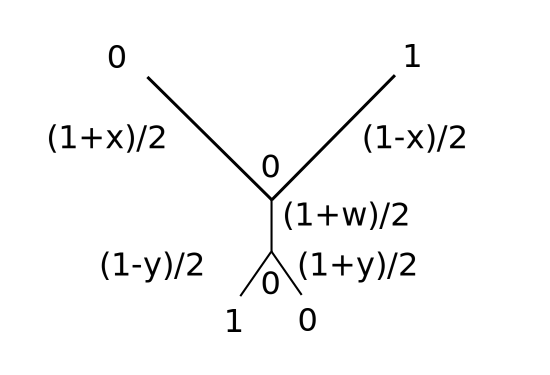
\includegraphics[width=.95\textwidth]{farris_like00}
\caption[short]{}
\end{subfigure}
\begin{subfigure}{.45\linewidth}
\centering
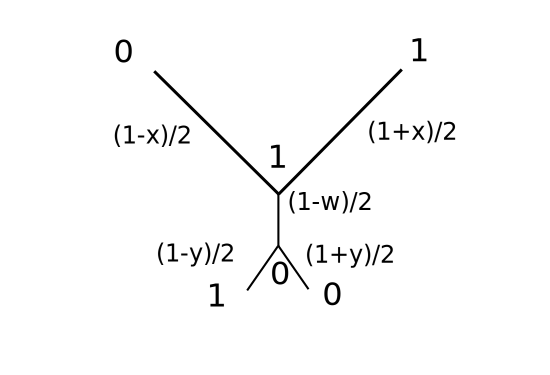
\includegraphics[width=.95\textwidth]{farris_like10}
\caption[short]{}
\end{subfigure}
\caption{
    Example likelihood computations on the Farris tree $\tau_1$ for fidelities $x$, $y$, and $w$.
    Edges labeled by the probability of substitution along that edge.
    In (a), we compute the product to obtain $\Pr(\ancestralStateColumn=\emptyset\mid \alignmentColumn=\{2,3\},\tau_1,t) = (1+x)(1-x)(1+y)(1-y)(1+w)/32$.
    In (b), the same process yields $\Pr(\ancestralStateColumn=\{1\}\mid \alignmentColumn=\{2,3\},\tau_1,t) = (1+x)(1-x)(1+y)(1-y)(1-w)/32$.
}
\label{fig:example_likelihoods}
\end{figure}

\begin{table}
\centering
\begin{tabular}{|l|ll|}
\multicolumn{3}{c}{$\Pr(\ancestralStateColumn=\ancestralSplit_k\mid \alignmentColumn=\siteSplit_j,\tau_1,t)$}\\
\hline
& \multicolumn{2}{|c|}{$\ancestralSplit_k$}\\
    \hline
    $\siteSplit_j$    &$\emptyset$                                &$\{2\}$  \\
    \hline
     $\emptyset$   &$(1+x)^2   (1+w)(1+y)^2$          &$(1+x)^2   (1-w)(1-y)^2$\\
     $\{1\}$       &$(1+x)(1-x)(1+w)(1+y)^2$          &$(1+x)(1-x)(1-w)(1-y)^2$\\
     $\{2\}$       &$(1+x)^2   (1+w)(1+y)(1-y)$       &$(1+x)^2   (1-w)(1+y)(1-y)$\\
     $\{3\}$       &$(1+x)(1-x)(1+w)(1+y)^2$          &$(1+x)(1-x)(1-w)(1-y)^2$\\
     $\{1,2\}$     &$(1+x)(1-x)(1+w)(1+y)(1-y)$       &$(1+x)(1-x)(1-w)(1+y)(1-y)$\\
     $\{1,3\}$     &$(1-x)^2   (1+w)(1+y)^2$          &$(1-x)^2   (1-w)(1-y)^2$\\
     $\{2,3\}$     &$(1+x)(1-x)(1+w)(1+y)(1-y)$       &$(1+x)(1-x)(1-w)(1+y)(1-y)$\\
     $\{1,2,3\}$   &$(1-x)^2   (1+w)(1+y)(1-y)$       &$(1-x)^2   (1-w)(1+y)(1-y)$\\
    \hline
    \hline
    &$\{1\}$                             &$\{1,2\}$  \\
    \hline
     $\emptyset$   &$(1-x)^2   (1-w)(1+y)^2$     &$(1-x)^2   (1+w)(1-y)^2$\\
     $\{1\}$       &$(1+x)(1-x)(1-w)(1+y)^2$     &$(1+x)(1-x)(1+w)(1-y)^2$\\
     $\{2\}$       &$(1-x)^2   (1-w)(1+y)(1-y)$  &$(1-x)^2   (1+w)(1+y)(1-y)$\\
     $\{3\}$       &$(1+x)(1-x)(1-w)(1+y)^2$     &$(1+x)(1-x)(1+w)(1-y)^2$\\
     $\{1,2\}$     &$(1+x)(1-x)(1-w)(1+y)(1-y)$  &$(1+x)(1-x)(1+w)(1+y)(1-y)$\\
     $\{1,3\}$     &$(1+x)^2   (1-w)(1+y)^2$     &$(1+x)^2   (1+w)(1-y)^2$\\
     $\{2,3\}$     &$(1+x)(1-x)(1-w)(1+y)(1-y)$  &$(1+x)(1-x)(1+w)(1+y)(1-y)$\\
     $\{1,2,3\}$   &$(1+x)^2   (1-w)(1+y)(1-y)$  &$(1+x)^2   (1+w)(1+y)(1-y)$\\
    \hline
\end{tabular}
\caption{Likelihood calculations for all site patterns $\siteSplit_j$ and internal states $\ancestralSplit_k$ of the Farris tree $\tau_1$.
All values multiplied by $1/32$.}
\label{tab:farris_likelihoods}
\end{table}

\begin{table}
\centering
\begin{tabular}{|l|ll|}
\multicolumn{3}{c}{$\Pr(\ancestralStateColumn=\ancestralSplit_k\mid \alignmentColumn=\siteSplit_j,\tau_2,t)$}\\
\hline
& \multicolumn{2}{|c|}{$\ancestralSplit_k$}\\
    \hline
    $\siteSplit_j$    &$\emptyset$                                &$\{2\}$  \\
    \hline
     $\emptyset$   &$(1+x)^2   (1+w)(1+y)^2$           &$(1+x)(1-x)(1-w)(1+y)(1-y)$\\
     $\{1\}$       &$(1+x)(1-x)(1+w)(1+y)^2$           &$(1-x)^2   (1-w)(1+y)(1-y)$\\
     $\{2\}$       &$(1+x)^2   (1+w)(1+y)(1-y)$        &$(1+x)(1-x)(1-w)(1-y)^2$\\
     $\{3\}$       &$(1+x)(1-x)(1+w)(1+y)^2$           &$(1+x)^2   (1-w)(1+y)(1-y)$\\
     $\{1,2\}$     &$(1+x)(1-x)(1+w)(1+y)(1-y)$        &$(1-x)^2   (1-w)(1-y)^2$\\
     $\{1,3\}$     &$(1-x)^2   (1+w)(1+y)^2$           &$(1+x)(1-x)(1-w)(1+y)(1-y)$\\
     $\{2,3\}$     &$(1+x)(1-x)(1+w)(1+y)(1-y)$        &$(1+x)^2   (1-w)(1-y)^2$\\
     $\{1,2,3\}$   &$(1-x)^2   (1+w)(1+y)(1-y)$        &$(1+x)(1-x)(1-w)(1-y)^2$\\
    \hline
    \hline
    &$\{1\}$                             &$\{1,2\}$  \\
    \hline
     $\emptyset$   &$(1+x)(1-x)(1-w)(1+y)(1-y)$        &$(1-x)^2   (1+w)(1-y)^2$\\
     $\{1\}$       &$(1+x)^2   (1-w)(1+y)(1-y)$        &$(1+x)(1-x)(1+w)(1-y)^2$\\
     $\{2\}$       &$(1+x)(1-x)(1-w)(1+y)^2$           &$(1-x)^2   (1+w)(1+y)(1-y)$\\
     $\{3\}$       &$(1-x)^2   (1-w)(1+y)(1-y)$        &$(1+x)(1-x)(1+w)(1-y)^2$\\
     $\{1,2\}$     &$(1+x)^2   (1-w)(1+y)^2$           &$(1+x)(1-x)(1+w)(1+y)(1-y)$\\
     $\{1,3\}$     &$(1+x)(1-x)(1-w)(1+y)(1-y)$        &$(1+x)^2   (1+w)(1-y)^2$\\
     $\{2,3\}$     &$(1-x)^2   (1-w)(1+y)^2$           &$(1+x)(1-x)(1+w)(1+y)(1-y)$\\
     $\{1,2,3\}$   &$(1+x)(1-x)(1-w)(1+y)^2$           &$(1+x)^2   (1+w)(1+y)(1-y)$\\
\hline
\end{tabular}
\caption{Likelihood calculations for all site patterns $\siteSplit_j$ and internal states $\ancestralSplit_k$ of the Felsenstein tree $\tau_2$.
All values multiplied by $1/32$.}
\label{tab:fels_likelihoods}
\end{table}

\begin{table}
\centering
\begin{tabular}{|l|ll|}
    \multicolumn{3}{c}{Farris tree ($\tau=\tau_1$)}\\
    \hline
    $\siteSplit_j$    & $\ancestralSplitPartition_j(\tau, t)$ & $\Pr(\ancestralSplitRV=\xi_j \mid \siteSplitRV=\siteSplit_j,\tau,t)$\\
    \hline
    $\emptyset$&
    $\emptyset$&
    $(1+x)^2   (1+w)(1+y)^2$\\
     $\{1\}$    &
    $\emptyset$&
    $(1+x)(1-x)(1+w)(1+y)^2$\\
     $\{2\}$    &
    $\emptyset$&
    $(1+x)^2   (1+w)(1+y)(1-y)$\\
     $\{3\}$    &
    $\emptyset$&
    $(1+x)(1-x)(1+w)(1+y)^2$\\
    $\{1,2\}$  &
    $\{\emptyset,\{1,2\}\}$&
    $(1+x)(1-x)(1+w)(1+y)(1-y)$\\
    $\{1,3\}$  &
    $\left\{\begin{array}{l}
                    \emptyset\\
                    \{1\}\\
                    \{1,2\}
                \end{array}\right.$&
    $\begin{array}{l}
                    (1-x)^2   (1+w)(1+y)^2\\
                    (1+x)^2   (1-w)(1+y)^2\\
                    (1+x)^2   (1+w)(1-y)^2
                \end{array}$\\
    $\{2,3\}$  &
                $\{\emptyset,\{1,2\}\}$&
                $(1+x)(1-x)(1+w)(1+y)(1-y)$\\
    $\{1,2,3\}$&
                $\{1,2\}$&
                $(1+x)^2   (1+w)(1+y)(1-y)$\\
    \hline
    \multicolumn{3}{c}{Felsenstein tree ($\tau=\tau_2$)}\\
    \hline
    $\siteSplit_j$    & $\ancestralSplitPartition_j(\tau, t)$ & $\Pr(\ancestralSplitRV=\xi_j \mid \siteSplitRV=\siteSplit_j,\tau,t)$\\
    \hline
    $\emptyset$       &$\emptyset$&$(1+x)^2   (1+w)(1+y)^2$\\
    $\{1\}$          &
    $\left\{\begin{array}{l}
                    \emptyset\\
                    \{1\}
                \end{array}\right.$&
    $\begin{array}{l}
                        (1+x)(1-x)(1+w)(1+y)^2\\
                        (1+x)^2   (1-w)(1+y)(1-y)
                    \end{array}$\\
      $\{2\}$          &
    $\left\{\begin{array}{l}
                    \emptyset\\
                    \{1\}
                \end{array}\right.$&
    $\begin{array}{l}
                    (1+x)^2   (1+w)(1+y)(1-y)\\
                    (1+x)(1-x)(1-w)(1+y)^2
                    \end{array}$\\
      $\{3\}$          &
    $\left\{\begin{array}{l}
                    \emptyset\\
                    \{2\}
                \end{array}\right.$&
    $\begin{array}{l}
                    (1+x)(1-x)(1+w)(1+y)^2\\
                    (1+x)^2   (1-w)(1+y)(1-y)
                    \end{array}$\\
     $\{1,2\}$         &
    $\left\{\begin{array}{l}
                    \{\emptyset,\{1,2\}\}\\
                    \{1\}
                \end{array}\right.$&
    $\begin{array}{l}
                    (1+x)(1-x)(1+w)(1+y)(1-y)\\
                    (1+x)^2   (1-w)(1+y)^2
                    \end{array}$\\
     $\{1,3\}$         &
    $\left\{\begin{array}{l}
                    \emptyset\\
                    \{\{1\},\{2\}\}\\
                    \{1,2\}
                \end{array}\right.$&
    $\begin{array}{l}
                    (1-x)^2   (1+w)(1+y)^2\\
                    (1+x)(1-x)(1-w)(1+y)(1-y)\\
                    (1+x)^2   (1+w)(1-y)^2
                    \end{array}$\\
      $\{2,3\}$        &
    $\left\{\begin{array}{l}
                    \{\emptyset,\{1,2\}\}\\
                    \{1\}\\
                    \{2\}
                \end{array}\right.$&
    $\begin{array}{l}
                    (1+x)(1-x)(1+w)(1+y)(1-y)\\
                    (1-x)^2   (1-w)(1+y)^2\\
                    (1+x)^2   (1-w)(1-y)^2
                    \end{array}$\\
     $\{1,2,3\}$       &
    $\left\{\begin{array}{l}
                    \{2\} \\
                    \{1,2\}
                \end{array}\right.$&
    $\begin{array}{l}
                    (1+x)(1-x)(1-w)(1+y)^2 \\
                    (1+x)^2   (1+w)(1+y)(1-y)
                    \end{array}$\\
    \hline
\end{tabular}
\caption{Likelihood calculations for all site patterns $\siteSplit_j$ and ancestral state partitions $\ancestralSplitPartition_j$ after maximizing over ancestral states on the Farris tree $\tau_1$ and the Felsenstein tree $\tau_2$.
All values multiplied by $1/32$.
Likelihoods with multiple entries have maxima determined by unknown branch length parameters.
See Tables~\ref{tab:farris_likelihoods} and~\ref{tab:fels_likelihoods} for full calculations.}
\label{tab:likelihoods}
\end{table}

\subsection*{Form of the likelihood}

Consider the Farris tree with arbitrary fidelities, i.e., $\tilde{t}=\{x_1,y_1,x_2,y_2,w\}$.
We now show that, in the case of the Farris tree, exchanging $x_1$ with $x_2$ and $y_1$ with $y_2$ does not change the value of the likelihood, and that constraining both the top two branch parameters to be equal and the bottom two branch parameters to be equal during inference obtains the same maximum likelihood estimate as in the case of arbitrary branch parameters.
Using the Hadamard transform, we calculate the generating probabilities on the Farris tree.
For site split $\emptyset$,
\begin{align*}
    \Pr(\siteSplitRV=\emptyset\mid \tau_1, \tilde{t}) & = \frac{1}{8} (1 + x_1x_2 +  y_1y_2 +  x_1y_1w + x_1y_2w + y_1x_2w + x_2y_2w + x_1y_1x_2y_2) \\
                                              & = \frac{1}{8} (1 + x_1x_2 +  y_1y_2 +  w[x_1y_1 + x_1y_2 + y_1x_2 + x_2y_2] + x_1y_1x_2y_2) \\
                                              & = \frac{1}{8} (1 + x_1x_2 +  y_1y_2 +  w[x_1 + x_2][y_1 + y_2] + x_1y_1x_2y_2).
\end{align*}
and this probability is unchanged when $x_1$ is exchanged with $x_2$ and $y_1$ is exchanged with $y_2$.
All other generating probabilities will differ only in the signs of each term.
For example, for site split $\{1\}$ we have
\begin{align*}
    \Pr(\siteSplitRV=\{1\}\mid \tau_1, \tilde{t}) & = \frac{1}{8} (1 - x_1x_2 +  y_1y_2 +  w[-x_1 + x_2][y_1 + y_2] - x_1y_1x_2y_2)
\end{align*}
and for site split $\{3\}$ we have
\begin{align*}
    \Pr(\siteSplitRV=\{3\}\mid \tau_1, \tilde{t}) & = \frac{1}{8} (1 - x_1x_2 +  y_1y_2 +  w[x_1 - x_2][y_1 + y_2] - x_1y_1x_2y_2)
\end{align*}
meaning if we exchange the values of $x_1$ and $x_2$ then these probabilities swap values.
The corresponding possibilities for the likelihood values are
\begin{align*}
    \Pr(\ancestralSplitRV=\emptyset \mid \siteSplitRV=\{1\}, \tau_1, \tilde{t}) &= \frac{1}{32}(1-x_1)(1+x_2)(1+w)(1+y_1)(1+y_2); \\
    \Pr(\ancestralSplitRV=\{1\} \mid \siteSplitRV=\{1\}, \tau_1, \tilde{t}) &= \frac{1}{32}(1+x_1)(1-x_2)(1-w)(1+y_1)(1+y_2); \\
    \Pr(\ancestralSplitRV=\{2\} \mid \siteSplitRV=\{1\}, \tau_1, \tilde{t}) &= \frac{1}{32}(1-x_1)(1+x_2)(1-w)(1-y_1)(1-y_2); \\
    \Pr(\ancestralSplitRV=\{1,2\} \mid \siteSplitRV=\{1\}, \tau_1, \tilde{t}) &= \frac{1}{32}(1+x_1)(1-x_2)(1+w)(1-y_1)(1-y_2);
\end{align*}
for site split $\{1\}$ and
\begin{align*}
        \Pr(\ancestralSplitRV=\emptyset \mid \siteSplitRV=\{3\}, \tau_1, \tilde{t}) &= \frac{1}{32}(1+x_1)(1-x_2)(1+w)(1+y_1)(1+y_2); \\
    \Pr(\ancestralSplitRV=\{1\} \mid \siteSplitRV=\{3\}, \tau_1, \tilde{t}) &= \frac{1}{32}(1-x_1)(1+x_2)(1-w)(1+y_1)(1+y_2); \\
    \Pr(\ancestralSplitRV=\{2\} \mid \siteSplitRV=\{3\}, \tau_1, \tilde{t}) &= \frac{1}{32}(1+x_1)(1-x_2)(1-w)(1-y_1)(1-y_2); \\
    \Pr(\ancestralSplitRV=\{1,2\} \mid \siteSplitRV=\{3\}, \tau_1, \tilde{t}) &= \frac{1}{32}(1-x_1)(1+x_2)(1+w)(1-y_1)(1-y_2);
\end{align*}
for site split $\{3\}$, which also both swap values when $x_1$ and $x_2$ are exchanged.

The same can be done for the splits $\{2\}$ and $\{1,2,3\}$ by exchanging $y_1$ and $y_2$ as well as $\{1,2\}$ and $\{1,3\}$ by exchanging both $x_1$ with $x_2$ and $y_1$ with $y_2$.
The split $\{1,3\}$ is unchanged by exchanging $x_1$ with $x_2$ and $y_1$ with $y_2$.

Since exchanging $x_1$ and $x_2$ does not change the value of the log-likelihood $\ell_{\tau_1,t^*}(\tau_1, \tilde{t})$, if there is a unique maximum of the log-likelihood we will have $x_1=x_2$ at the maximum.
An analogous statement holds for $y_1$ and $y_2$.
It remains to show that the joint inference procedure maximizing \eqref{eq:profile_likelihood} results in a unique estimate of $t$.
Without loss of generality, we focus on the single parameter $x_1$ and show we obtain a unique maximum when performing joint inference; similar arguments hold for the remaining parameters.
We decompose the likelihood into the entropy and partial likelihood terms as in \eqref{eq:log_likelihood_simplified}.
By Gibbs's inequality, the entropy term $\shannonDivergence_{\tau^*,t^*}(\tau^*,t)$ has a unique maximum over $t$---namely $t^*$.
For the general case of $\tilde{t}=\{x_1, y_2, x_1, y_2, w\}$, we can compute the partial likelihood $\tilde{\ell}_{\tau^*,t^*}(\tau^*, t)$ as in Table~\ref{tab:farris_likelihoods}.
Clearly this partial likelihood will be of the form $g(x_1) = p\log(1+x_1) + (1-p)\log(1-x_1)$ with $0 \le p \le 1$, which, by the second derivative test, is concave for $x_1\in[0,1]$ and thus has a unique maximum.
Since both summands of the likelihood are concave on $x_1\in[0,1]$, the likelihood is as well, and there exists a single $x_1\in[0,1]$ maximizing the likelihood.
Given this and the symmetry of the likelihood, we let $x_1=x_2=x$ and $y_1=y_2=y$.
The Felsenstein tree does not admit this property, but, since we are interested in a lower bound for this tree, we simplify the objective function by constraining $x_1=x_2$ and $y_1=y_2$ similarly.

\subsection*{Theorems and proofs}

\topoInconsist*

\begin{proof}
In general,
$$
\max_{t} \ \ell_{\tau^*,t^*}(\tau, t) \le
    \shannonDivergence_{\tau^*,t^*}(\tau^*,t^*)
    + \tilde{\ell}_{\tau^*,t^*}(\tau, \hat{t})
$$
is an upper bound for the joint maximum of \eqref{eq:log_likelihood_simplified} using Gibbs's inequality
$$
\shannonDivergence_{\tau^*,t^*}(\tau,t) \le \shannonDivergence_{\tau^*,t^*}(\tau^*,t^*)
$$
and
$$
\hat{t} = \argmax_{t} \ \tilde{\ell}_{\tau^*,t^*}(\tau, t).
$$
Similarly,
$$
\max_{t} \ \ell_{\tau^*,t^*}(\tau, t) \ge
    \shannonDivergence_{\tau^*,t^*}(\tau,\hat{t})
    + \tilde{\ell}_{\tau^*,t^*}(\tau, \hat{t})
$$
is a lower bound.

Assume $\tau^*=\tau_1$.
The Farris tree log-likelihood takes one of three values depending on branch lengths, which is due to site split $\{1,3\}$ (see the upper table of Table~\ref{tab:likelihoods}).

We write out the case for the ancestral state split $\{1\}$, and show the other two cases follow a similar argument.
Directly substituting calculations from Table~\ref{tab:sitepatprob} and Table~\ref{tab:likelihoods} where $\tau = \tau_1$ in \eqref{eq:site_pattern_profile_likelihood_mean}, the log-likelihood is, suppressing normalizing constants $-\log 8$ (from the first additive term of \eqref{eq:site_pattern_profile_likelihood_mean}) and $-\log 32$ (from the second),
\begin{align}
    \label{eq:farris_likelihood}
    \ell_{\tau_1,t^*}(\tau_1, t)
    &=        p_{\emptyset}  \cdot\log(1+x^2+y^2+4xyw+x^2y^2) \nonumber \\
    &\qquad + p_{1}          \cdot\log(1-x^2+y^2-x^2y^2) \nonumber \\
    &\qquad + p_{2}          \cdot\log(1+x^2-y^2-x^2y^2) \nonumber \\
    &\qquad + p_{3}          \cdot\log(1-x^2+y^2-x^2y^2) \nonumber \\
    &\qquad + p_{12}         \cdot\log(1-x^2-y^2+x^2y^2) \nonumber \\
    &\qquad + p_{13}         \cdot\log(1+x^2+y^2-4xyw+x^2y^2) \nonumber \\
    &\qquad + p_{23}         \cdot\log(1-x^2-y^2+x^2y^2) \nonumber \\
    &\qquad + p_{123}        \cdot\log(1+x^2-y^2-x^2y^2) \nonumber \\
    &\qquad + p_{\emptyset}  \cdot\log((1+x)^2   (1+w)(1+y)^2) \nonumber \\
    &\qquad + p_{1}          \cdot\log((1+x)(1-x)(1+w)(1+y)^2) \nonumber \\
    &\qquad + p_{2}          \cdot\log((1+x)^2   (1+w)(1+y)(1-y)) \nonumber \\
    &\qquad + p_{3}          \cdot\log((1+x)(1-x)(1+w)(1+y)^2) \nonumber \\
    &\qquad + p_{12}         \cdot\log((1+x)(1-x)(1+w)(1+y)(1-y)) \nonumber \\
    &\qquad + p_{13}         \cdot\log((1+x)^2   (1-w)(1+y)^2) \nonumber \\
    &\qquad + p_{23}         \cdot\log((1+x)(1-x)(1+w)(1+y)(1-y)) \nonumber \\
    &\qquad + p_{123}        \cdot\log((1+x)^2   (1+w)(1+y)(1-y)).
\end{align}
Our plan is to simplify the likelihood to remove log-of-quadratic terms of $x,y,$ and $w$, obtaining a likelihood that has a closed-form maximum in each variable.
To bound the generating probabilities, we use the facts that, for $x,y\in[0,1]$,
\begin{align*}
p_{12} = p_{23} = 1-x^2-y^2+x^2y^2 & = (1+x)(1-x)(1+y)(1-y) \\
p_{1} = p_{3} = 1-x^2+y^2-x^2y^2 & = (1+x)(1-x)(1+y^2) \le (1+x)(1-x)(1+y) \\
p_{2} = p_{123} = 1+x^2-y^2-x^2y^2 & = (1+x^2)(1+y)(1-y) \le (1+x)(1+y)(1-y).
\end{align*}
To bound the remaining $p_{\emptyset}$ and $p_{13}$, we use
\begin{align*}
1+x^2+y^2+x^2y^2 & = (1+x^2)(1+y^2) \le (1+x)(1+y) \\
4xy & = 2x \cdot 2y \le (1+x^2)(1+y^2) \le (1+x)(1+y)
\end{align*}
so that the $p_{\emptyset}$ term is bounded as
\begin{align*}
    p_{\emptyset} & = \log(1+x^2+y^2+4xyw+x^2y^2) \\
                  & \le \log(1+x^2+y^2+4xy+x^2y^2) \\
                  & \le \log(2(1+x)(1+y))
\end{align*}
and $p_{13}$ is bounded as
\begin{align*}
    p_{13} & = \log(1+x^2+y^2-4xyw+x^2y^2) \\
                  & \le \log(1+x^2+y^2+x^2y^2) \\
                  & \le \log((1+x)(1+y)).
\end{align*}
Factoring and making these substitutions (again, under the assumption that the ancestral state split is $\{1\}$) results in
\begin{align*}
&    \ell_{\tau_1,t^*}(\tau_1, t) \\
&\qquad \le      p_{\emptyset}  \cdot\log(2(1+x)(1+y))
+ p_{1}          \cdot\log((1+x)(1-x)(1+y)) \\
    &\qquad\qquad + p_{2}          \cdot\log((1+x)(1+y)(1-y))
+ p_{3}          \cdot\log((1+x)(1-x)(1+y)) \\
    &\qquad\qquad + p_{12}         \cdot\log((1+x)(1-x)(1+y)(1-y))
+ p_{13}         \cdot\log((1+x)(1+y)) \\
    &\qquad\qquad + p_{23}         \cdot\log((1+x)(1-x)(1+y)(1-y))
+ p_{123}        \cdot\log((1+x)(1+y)(1-y)) \\
    &\qquad\qquad + p_{\emptyset}  \cdot\log((1+x)^2   (1+w)(1+y)^2)
+ p_{1}          \cdot\log((1+x)(1-x)(1+w)(1+y)^2) \\
    &\qquad\qquad + p_{2}          \cdot\log((1+x)^2   (1+w)(1+y)(1-y))
+ p_{3}          \cdot\log((1+x)(1-x)(1+w)(1+y)^2) \\
    &\qquad\qquad + p_{12}         \cdot\log((1+x)(1-x)(1+w)(1+y)(1-y))
+ p_{13}         \cdot\log((1+x)^2   (1-w)(1+y)^2) \\
    &\qquad\qquad + p_{23}         \cdot\log((1+x)(1-x)(1+w)(1+y)(1-y))
+ p_{123}        \cdot\log((1+x)^2   (1+w)(1+y)(1-y)) \\
&\qquad =      p_{\emptyset}  \cdot\log(2)
+ \log(1+x)
+ (p_{1}+p_{3}+p_{12}+p_{23})\cdot\log(1-x) \\
&\qquad\qquad + \log(1+y)
+ (p_{2}+p_{12}+p_{23}+p_{123})\cdot\log(1-y) \\
&\qquad\qquad + (2-p_{1}-p_{3}-p_{12}-p_{23})\cdot\log(1+x)
+ (p_{1}+p_{3}+p_{12}+p_{23})\cdot\log(1-x) \\
&\qquad\qquad + (2-p_{2}-p_{12}-p_{23}-p_{123})\cdot\log(1+y)
+ (p_{2}+p_{12}+p_{23}+p_{123})\cdot\log(1-y) \\
&\qquad\qquad + (1-p_{13})\cdot\log(1+w)
+ p_{13}\cdot\log(1-w) \\
&\qquad =      p_{\emptyset}  \cdot\log(2)
+ (3-p_{1}-p_{3}-p_{12}-p_{23})\cdot\log(1+x)
+ 2(p_{1}+p_{3}+p_{12}+p_{23})\cdot\log(1-x) \\
&\qquad\qquad + (3-p_{2}-p_{12}-p_{23}-p_{123})\cdot\log(1+y)
+ 2(p_{2}+p_{12}+p_{23}+p_{123})\cdot\log(1-y) \\
&\qquad\qquad + (1-p_{13})\cdot\log(1+w)
+ p_{13}\cdot\log(1-w).
\end{align*}
To simplify, let
\begin{equation}
    \begin{aligned}
        a_{1} &= 3-p_{1}-p_{3}-p_{12}-p_{23}, \\
        a_{2} &= 2(p_{1}+p_{3}+p_{12}+p_{23}), \\
        a_{3} &= 3-p_{2}-p_{12}-p_{23}-p_{123}, \\
        a_{4} &= 2(p_{2}+p_{12}+p_{23}+p_{123}), \\
    \end{aligned}
    \label{eq:a_const}
\end{equation}
so that
\begin{equation*}
\begin{split}
&    \ell_{\tau_1,t^*}(\tau_1, t) \\
&\qquad \le      p_{\emptyset}  \cdot\log(2)
+ a_{1}\cdot\log(1+x)
+ a_{2}\cdot\log(1-x)
+ a_{3}\cdot\log(1+y) \\
&\qquad\qquad + a_{4}\cdot\log(1-y)
+ (1-p_{13})\cdot\log(1+w)
+ p_{13}\cdot\log(1-w).
\end{split}
\end{equation*}
Maximizing over the unknown terms yields
$$
\hat{x} = \frac{a_{1}-a_{2}}{a_{1}+a_{2}}, \ \hat{y} = \frac{a_{3}-a_{4}}{a_{3}+a_{4}}, \ \hat{w} = 1-2p_{13}.
$$
Trivially $0 \le \hat{w} \le 1$ and $\hat{x}, \hat{y} \le 1$.
We check that $\hat{x}, \hat{y} \ge 0$ to ensure these maxima are valid.
For $\hat{x} \ge 0$ we need $a_1 \ge a_2$; letting
$$
\tilde{p} = p_{1}+p_{3}+p_{12}+p_{23}
$$
we have from \eqref{eq:a_const} that $a_1 \ge a_2$ only if $3 \ge 3\tilde{p}$.
Since $\tilde{p} = 1/8\cdot(4-4(x^*)^2)$, we have $0 \le \tilde{p} \le 1/2$ implying $\hat{x} \ge 0$.
The same approach works for $\hat{y}$.
The upper bound for the likelihood is then maximized at
\begin{align}
\begin{split}
&    \ell_{\tau_1,t^*}(\tau_1, t) \\
&\qquad\le      p_{\emptyset}  \cdot\log(2)
+ a_{1}\cdot\log\frac{2a_{1}}{a_{1}+a_{2}}
+ a_{2}\cdot\log\frac{2a_{2}}{a_{1}+a_{2}}
+ a_{3}\cdot\log\frac{2a_{3}}{a_{3}+a_{4}} \\
&\qquad\qquad + a_{4}\cdot\log\frac{2a_{4}}{a_{3}+a_{4}}
+ (1-p_{13})\cdot\log(2(1-p_{13}))
+ p_{13}\cdot\log(2p_{13}) \\
&\qquad := C^{1}_{\tau_1,\tau_1}(x^*, y^*).
\end{split}
\label{eq:farris-upper-bound}
\end{align}

The other two possible ancestral state splits for the likelihood of the site split $\{1,3\}$ admit similar simplifications.
The upper bound in \eqref{eq:farris-upper-bound} is for the ancestral state split $\{1\}$.
For the ancestral state split $\emptyset$ we see the upper bound will be the same except we lose a $(1+x)^2$ term, gain a $(1-x)^2$ term, lose a $(1-w)$ term, and gain a $(1+w)$ term.
In this case, all terms involving $w$ simplify to $\log(1+w)$, maximized at $\hat{w}=1$.
For the constants above, $a_{1}$ is the multiplier for the $\log(1+x)$ term and $a_{2}$ for the $\log(1-x)$ term meaning that exchanging the above quadratic $x$ terms yields new constants
\begin{equation}
    \begin{aligned}
        a_{1}' &= a_{1}-2p_{13}, \\
        a_{2}' &= a_{2}+2p_{13}, \\
    \end{aligned}
    \label{eq:a_const_prime_x}
\end{equation}
for site split $\emptyset$ and
\begin{equation}
    \begin{aligned}
        a_{3}' &= a_{3}-2p_{13}, \\
        a_{4}' &= a_{4}+2p_{13}, \\
    \end{aligned}
    \label{eq:a_const_prime_y}
\end{equation}
for site split $\{1,2\}$.
To bound the case of $\ancestralSplitPartition_j(\tau_1, t) = \emptyset$,
\begin{align*}
&    \ell_{\tau_1,t^*}(\tau_1, t) \\
&\qquad\le      p_{\emptyset}  \cdot\log(2)
+ a_{1}'\cdot\log\frac{2a_{1}'}{a_{1}'+a_{2}'}
+ a_{2}'\cdot\log\frac{2a_{2}'}{a_{1}'+a_{2}'} \\
&\qquad\qquad + a_{3}\cdot\log\frac{2a_{3}}{a_{3}+a_{4}}
+ a_{4}\cdot\log\frac{2a_{4}}{a_{3}+a_{4}}
+ \log(2) \\
&\qquad := C^{2}_{\tau_1,\tau_1}(x^*, y^*),
\end{align*}
and, for the case of $\ancestralSplitPartition_j(\tau_1, t) = \{1,2\}$,
\begin{align*}
&    \ell_{\tau_1,t^*}(\tau_1, t) \\
&\qquad\le      p_{\emptyset}  \cdot\log(2)
+ a_{1}\cdot\log\frac{2a_{1}}{a_{1}+a_{2}}
+ a_{2}\cdot\log\frac{2a_{2}}{a_{1}+a_{2}} \\
&\qquad\qquad+ a_{3}'\cdot\log\frac{2a_{3}'}{a_{3}'+a_{4}'}
+ a_{4}'\cdot\log\frac{2a_{4}'}{a_{3}'+a_{4}'}
+ \log(2) \\
&\qquad := C^{3}_{\tau_1,\tau_1}(x^*, y^*).
\end{align*}

We now need to check that
$$
\hat{x} = \frac{a_{1}'-a_{2}'}{a_{1}'+a_{2}'}, \ \hat{y} = \frac{a_{3}'-a_{4}'}{a_{3}'+a_{4}'}
$$
are both between zero and one.
Using a similar argument as that where $\ancestralSplitPartition_j(\tau_1, t) = \{1,3\}$, we only need to show $a_1' \ge a_2'$, which is true if $3-2p_{13} \ge 3\tilde{p}+2p_{13}$.
Some rearranging and the fact that $0 \le \tilde{p} \le 1/2$ shows this is equivalent to showing $p_{13} \le 3/8$.
Using Table~\ref{tab:sitepatprob} and $t^*$,
$$
p_{13} = \frac{1}{8}\left(1 + (x^*)^2 + (y^*)^2 - 4x^*(y^*)^2 + (x^*)^2(y^*)^2\right),
$$
meaning we are interested in whether
\begin{equation}
1 + (x^*)^2 + (y^*)^2 - 4x^*(y^*)^2 + (x^*)^2(y^*)^2 \le 3.
\label{eq:generating_ineq}
\end{equation}
We see that
\begin{equation}
1 + (x^*)^2 + (y^*)^2 - 4x^*(y^*)^2 + (x^*)^2(y^*)^2 \le 3 \iff (y^*)^2\left(1 - 4x^* + (x^*)^2\right) \le 2 - (x^*)^2
\label{eq:lenny}
\end{equation}
and that
\begin{align*}
(y^*)^2\left(1 - 4x^* + (x^*)^2\right) &\le (y^*)^2\left(1 - 2x^* + (x^*)^2\right) \\
                                       &=   (y^*)^2\left(1 - x^*\right)^2 \\
                                       &\le        \left(1 - x^*\right)^2 \\
                                       &\le              2 - (x^*)^2,
\end{align*}
with the last inequality holding if $0 \le x^* \le 1$, showing that \eqref{eq:lenny} holds.
Thus, $p_{13} \le 3/8$ and our $\hat{x}$ and $\hat{y}$ are valid.

All bounds are functions only of $x,y$ through the true generating probabilities $x^*, y^*$.
Call the upper bound
$$
C_0(x^*, y^*) := \max\left(C^{1}_{\tau_1,\tau_1}(x^*, y^*), C^{2}_{\tau_1,\tau_1}(x^*, y^*), C^{3}_{\tau_1,\tau_1}(x^*, y^*)\right).
$$

We construct a similar lower bound on the Felsenstein tree partial likelihood.
In the Felsenstein case, there are many more optimal internal states depending on branch lengths than in the Farris case (see the lower table of Table~\ref{tab:likelihoods}).
We first bound the entire likelihood below and then proceed with joint inference.
To obtain a lower bound for the likelihood we replace $1+w$ with $1-w$ in Table~\ref{tab:likelihoods} for $\tau = \tau_2$; in this case, we resolve many of the ambiguous likelihood terms.
For example, for site split $\{1,2\}$, after we replace the $1+w$ term for $\ancestralSplitPartition_j(\tau, t)=\{\emptyset, \{1,2\}\}$ with $1-w$, we have
$$
\max\left((1+x)^2 (1-w)(1+y)^2, (1+x)(1-x)(1-w)(1+y)(1-y)\right)
$$
where since
$$
(1+x)^2 (1-w)(1+y)^2 > (1+x)(1-x)(1-w)(1+y)(1-y),
$$
the maximum for this site split can be bounded below by $(1+x)^2 (1-w)(1+y)^2$.
For the other site splits we consider two cases.
If $(1+x)(1-y) > (1-x)(1+y)$, then
$$
(1+x)^2(1-w)(1+y)(1-y) > (1+x)(1-x)(1-w)(1+y)^2
$$
meaning the cases $\{1\}, \{2\}, \{3\}$ and $\{1,2,3\}$ will have likelihoods bounded below by
$$
(1+x)^2(1-w)(1+y)(1-y).
$$
For the cases $\{1,3\}$ and $\{2,3\}$ and the same condition, we have
$$
(1+x)^2(1-w)(1-y)^2 > (1-x)^2(1-w)(1+y)^2
$$
and
$$
(1+x)^2(1-w)(1-y)^2 > (1+x)(1-x)(1-w)(1+y)(1-y),
$$
yielding lower bounds of
$$
(1+x)^2(1-w)(1-y)^2
$$
in these cases.
The partial likelihood in this case is then bounded below by
\begin{align*}
    \tilde{\ell}_{\tau_1,t^*}(\tau_2, t)
    &\ge      p_{\emptyset}  \cdot\log((1+x)^2   (1-w)(1+y)^2) \\
    &\qquad + p_{1}          \cdot\log((1+x)^2   (1-w)(1+y)(1-y)) \\
    &\qquad + p_{2}          \cdot\log((1+x)^2   (1-w)(1+y)(1-y)) \\
    &\qquad + p_{3}          \cdot\log((1+x)^2   (1-w)(1+y)(1-y)) \\
    &\qquad + p_{12}         \cdot\log((1+x)^2   (1-w)(1+y)^2) \\
    &\qquad + p_{123}        \cdot\log((1+x)^2   (1-w)(1+y)(1-y))\\
    &\qquad + p_{13}         \cdot\log((1+x)^2   (1-w)(1-y)^2) \\
    &\qquad + p_{23}         \cdot\log((1+x)^2   (1-w)(1-y)^2).
\end{align*}
When $(1+x)(1-y) < (1-x)(1+y)$, similar arguments yield the lower bound
\begin{align*}
    \tilde{\ell}_{\tau_1,t^*}(\tau_2, t)
    &\ge      p_{\emptyset}  \cdot\log((1+x)^2    (1-w)(1+y)^2) \\
    &\qquad + p_{1}          \cdot\log((1+x)(1-x)(1-w)(1+y)^2) \\
    &\qquad + p_{2}          \cdot\log((1+x)(1-x)(1-w)(1+y)^2) \\
    &\qquad + p_{3}          \cdot\log((1+x)(1-x)(1-w)(1+y)^2) \\
    %See above.
    &\qquad + p_{12}         \cdot\log((1+x)^2    (1-w)(1+y)^2) \\
    &\qquad + p_{123}        \cdot\log((1+x)(1-x)(1-w)(1+y)^2)\\
    &\qquad + p_{13}         \cdot\log((1-x)^2    (1-w)(1+y)^2) \\
    &\qquad + p_{23}         \cdot\log((1-x)^2    (1-w)(1+y)^2).
\end{align*}
Letting
$$
b = p_{1}+p_{2}+p_{3}+p_{123}
$$
yields
$$
    \tilde{\ell}_{\tau_1,t^*}(\tau_2, t)
    \ge      2\cdot\log(1+x)
    + (2-b)  \cdot\log(1+y)
    + b      \cdot\log(1-y)
    + \log(1-w)
$$
for the first lower bound, and we get the equivalent expression for the second lower bound by exchanging $x$ and $y$.
Maximizing either lower bound over $t$, we obtain
$$
\tilde{\ell}_{\tau_1,t^*}(\tau_2, t)
\ge      2\cdot\log(2)
+ (2-b)  \cdot\log(2-b)
+ b      \cdot\log(b),
$$
i.e., the maximum is achieved at $\{1,1-b,0\}$.
Our lower bound is
$$
C_1(x^*, y^*) := \shannonDivergence_{\tau_1,t^*}(\tau_2,\{1,1-b,0\}) + 2\cdot\log(2) + (2-b)\cdot\log(2-b) + b\cdot\log(b).
$$
See Fig.~\ref{fig:inconsistency-farris} for the values of $0 < x^*, y^* < 1$ where $C_1(x^*, y^*) > C_0(x^*, y^*)$ and joint inference is inconsistent.
\end{proof}

\restrictedBranchInconsist*

\begin{proof}
Recalling Table~\ref{tab:likelihoods} for the Farris tree $\tau = \tau_1$, the likelihood can take one of three forms corresponding to which ancestral state for $\siteSplit_j=\{1,3\}$ maximizes the likelihood over $(x,y,w)$.
If $x=x^*$ and $y=y^*$ are fixed, by collapsing like terms and ignoring terms with only $x^*$ and $y^*$, the log-likelihood in \eqref{eq:farris_likelihood} as a function of $w$ is
\begin{align*}
    \ell_{\tau_1,t^*}(\tau_1, w)
    &\sim     p_{\emptyset}  \cdot\log(1+(x^*)^2+(y^*)^2+4x^*y^*w+(x^*)^2(y^*)^2) \\
    &\qquad + p_{13}         \cdot\log(1+(x^*)^2+(y^*)^2-4x^*y^*w+(x^*)^2(y^*)^2) \\
    &\qquad + (1 - p_{13})\cdot\log(1+w) \\
    &\qquad + p_{13}\cdot\log(1-w)
\end{align*}
where $\sim$ denotes equality up to an additive constant.
Similarly, the other two possibilities for the likelihood both satisfy
\begin{align*}
    \ell_{\tau_1,t^*}(\tau_1, w)
    &\sim     p_{\emptyset}  \cdot\log(1+(x^*)^2+(y^*)^2+4x^*y^*w+(x^*)^2(y^*)^2) \\
    &\qquad + p_{13}         \cdot\log(1+(x^*)^2+(y^*)^2-4x^*y^*w+(x^*)^2(y^*)^2) \\
    &\qquad + \log(1+w).
\end{align*}
Since
$$
\log(1+w) \geq (1 - p_{13})\cdot\log(1+w) + p_{13}\cdot\log(1-w)
$$
with equality only when $w=0$, the second likelihood is the likelihood with the maximum-likelihood ancestral state, and so we only analyze that case.

Now substitute in values for $p_{\emptyset}$ and $p_{13}$ from Table~\ref{tab:sitepatprob}.
Simplifying, the likelihood can be written
$$
\ell(w) = \alpha_1\log(\beta+\gamma w) + \alpha_2\log(\beta-\gamma w) + \log(1+w)
$$
where
$$
\alpha_1 := \alpha_1(x^*, y^*) = \frac{1}{8} \left(1+(x^*)^2+(y^*)^2+4x^*(y^*)^2+(x^*)^2(y^*)^2\right),
$$
$$
\alpha_2 := \alpha_2(x^*, y^*) = \frac{1}{8}\left(1+(x^*)^2+(y^*)^2-4x^*(y^*)^2+(x^*)^2(y^*)^2\right),
$$
$$
\beta := \beta(x^*, y^*) = 1+(x^*)^2+(y^*)^2+(x^*)^2(y^*)^2,
$$
$$
\gamma := \gamma(x^*, y^*) = 4x^*y^*.
$$
Since $x^*$ and $y^*$ fall between zero and one, we make use of the inequalities (excepting the cases of $x^*=y^*=0$ and $x^*=y^*=1$)
$$
\alpha_1 > \alpha_2
$$
and
$$
\beta > \gamma.
$$
% Not sure if I need to show this, but if x and y aren't 1 it's 1+x^2+y^2+x^2y^2 > 4xy => (1+x^2)(1+y^2) > 4xy and 1+x^2 > 2x, 1+y^2 > 2y qed
The derivative of the log-likelihood with respect to $w$ is
$$
\ell'(w) := \frac{d}{dw} \ell(w) = \frac{\alpha_1 \gamma}{\beta+\gamma w} - \frac{\alpha_2 \gamma}{\beta-\gamma w} + \frac{1}{1+w}.
$$
The inequality $\beta > \gamma$ implies that this function stays finite and that, when considering $\ell'(w) \lessgtr 0$, we equivalently consider $f(w) \lessgtr 0$ where $f$ is the quadratic function
\begin{align*}
f(w) &= (w)^2\cdot(-\gamma^2\alpha_1-\gamma^2\alpha_2-\gamma^2) \\
      &\qquad + w\cdot(\gamma\alpha_1\beta-\gamma^2\alpha_1-\gamma\alpha_2\beta-\gamma^2\alpha_2) \\
      &\qquad + (\gamma\alpha_1\beta-\gamma\alpha_2\beta+\beta^2).
\end{align*}
% Note from das: b^2 - 4ac is always \ge 0 by \alpha_1 > \alpha_2, so b^2 - 4ac can only be zero if b is zero and a or c is zero. c is never zero, so this means a must be zero for this to happen, which only occurs if \gamma = 0, i.e., if x or y is zero.
Excepting all the cases where $x^*=0$ or where $y^*=0$, this implies $\ell'$ has two zeros according to the quadratic formula.
Because $\alpha_1 > \alpha_2$ we have $\ell'(0) > 0$, and thus $\ell$ is increasing at $w=0$.
This implies that if the smaller of the zeros of $f(w)$ is greater than one, then $\hat{w} \equiv 1$.
Using the quadratic formula with
$$
a = -\gamma^2 \alpha_1 - \gamma^2 \alpha_2 - \gamma^2,
$$
$$
b = \gamma \alpha_1 \beta - \gamma^2\alpha_1 - \gamma \alpha_2 \beta - \gamma^2 \alpha_2,
$$
$$
c = \gamma \alpha_1 \beta - \gamma \alpha_2 \beta + \beta^2,
$$
the smaller zero is
$$
\hat{w} = \frac{-b - \sqrt{b^2 - 4ac}}{2a},
$$
which is a function of the generating parameters $x^*$ and $y^*$.
We see that $a \le 0$ and, by a small calculation, $2a+b \leq 0$.
With this we have,
$$
\hat{w} \ge 1 \iff
|2a + b| \leq \sqrt{b^2 - 4ac} \iff
%-b - \sqrt{b^2 - 4ac} \le 2a,
%0 \ge -b - 2a \le \sqrt{b^2 - 4ac},
%b^2 + 4ab + 4a^2 \le b^2 - 4ac,
%a^2 + ab + ac \le 0,
a + b + c \ge 0.
$$
Using
$$
\alpha_1 + \alpha_2 = \frac{1}{4}\beta
$$
and
$$
\alpha_1 - \alpha_2 = x^*(y^*)^2,
$$
and simplifying as functions of $\gamma$ and $\beta$ shows that $a + b + c \ge 0$ is equivalent to
\begin{equation}
\label{eq:restricted-bl-result}
%\beta^2-\gamma^2-2\gamma^2\alpha_1-2\gamma^2\alpha_2+2\gamma\alpha_1\beta-2\gamma\alpha_2\beta \ge 0.
-\gamma^2\left(1 + \frac{1}{2}\beta\right) + 2\gamma\beta x^*(y^*)^2 + \beta^2 \ge 0.
\end{equation}
\end{proof}

\generalBranchInconsist*

\begin{proof}
In the general case, $\hat{w}$ is a function of $x^*$, $y^*$, $\hat{x}$, and $\hat{y}$.
From the previous section, $\hat{w}$ is given by the quadratic formula, though now with $\gamma$ and $\beta$ as functions of $\hat{x}$ and $\hat{y}$ instead of $x^*$ and $y^*$.
Assume we know $\hat{x}$ and $\hat{y}$ as functions of $x^*$ and $y^*$ only.
The same derivation as for \eqref{eq:restricted-bl-result} further yields
\begin{equation}
\label{eq:general-bl-result}
-\gamma^2(\hat{x}, \hat{y})\left(1 + \frac{1}{2}\beta\right) + 2\gamma(\hat{x}, \hat{y})\beta(\hat{x}, \hat{y})x^*(y^*)^2 + \beta^2(\hat{x}, \hat{y}) \ge 0
\end{equation}
where, since $\alpha_1$ and $\alpha_2$ are still functions of $x^*$ and $y^*$, $\left(1+1/2\cdot\beta\right)$ and $x^*(y^*)^2$ from \eqref{eq:restricted-bl-result} remain unchanged.
Given the bounds
$$
\gamma_{L} \le \gamma(\hat{x}, \hat{y}) \le \gamma_{U}
$$
and
$$
\beta_{L} \le \beta(\hat{x}, \hat{y}),
$$
if
$$
-\gamma_{U}^2\left(1 + \frac{1}{2}\beta\right) + 2\gamma_{L}\beta_{L}x^*(y^*)^2 + \beta_{L}^2 \ge 0,
$$
then \eqref{eq:general-bl-result} holds, and this is an inequality involving only $x^*$ and $y^*$.
\end{proof}
To get a sense of the region of overestimation, Fig.~\ref{fig:bl-loose-inconsistency} plots an intermediate case.
\subsection*{Empirical validation}

We use basin-hopping \citep{Wales1997} implemented in \texttt{scipy} \citep{Jones2001} to obtain the plots in Figs.~\ref{fig:bl-general-inconsistency}, \ref{fig:bl-general-marginal}, and \ref{fig:bl-general-bias}.
This method randomly perturbs candidate solutions and accepts or rejects them based on the nearby likelihood surface, eventually obtaining an estimate of the ``global'' optimum.
While it is not guaranteed to always obtain a global optimum---or even always converge---its implementation here leads us to believe that we can estimate $\hat{w}$ as well as any optimization method available.

We take various safeguards to ensure convergence and stability of the procedure.
Since this method involves randomness, we take precautions to not evaluate the likelihood near or outside of boundary conditions, i.e., when $x^*$ or $y^*$ are either $0$ or $1$.
As is apparent from Table~\ref{tab:sitepatprob}, if $0 < x^*, y^* < 1$ and we try to evaluate the candidate $\hat{x}=\hat{y}=\hat{w}=1$ we have a likelihood of exactly zero.
Worse still, in Table~\ref{tab:likelihoods} for the Farris tree, in the cases of $\{2\}, \{1,2\}, \{2,3\},$ and $\{1,2,3\}$, any attempt to evaluate $\hat{y}=1$ will similarly yield a zero likelihood.
In these cases of zero likelihood, methods that evaluate many candidate parameter values can fail to converge when near these boundaries.
We sidestep these computational issues by restricting ourselves to the region $x^*,y^*\in [10^{-2},1-10^{-2}]^2$.

We initialize our optimization procedure at the true branch parameters $t^*=\{x^*,y^*,x^*,y^*,y^*\}$.
Because our analysis shows that $\hat{w}$ can be equal to one when $x^*$ and $y^*$ are small, and local optimization may have a hard time obtaining this value if our initial guess is small, we perform two maximizations, one with $w=1$ fixed and one where $w$ is estimated.
We take the value of $\hat{w}$ with the larger objective function as our estimate.

\begin{figure}
\centering
% obtained by running
% python joint_inf_plot.py --empirical --general-branch-lengths --delta .01 --plot-name figures/w-hat-empirical-01-marginal.svg --out-pkl-name figures/w-hat-empirical-01-marginal.pkl --n-jobs 16 --marginal
% or
% python joint_inf_plot.py --empirical --general-branch-lengths --plot-name figures/w-hat-empirical-01-marginal.svg --in-pkl-name figures/w-hat-empirical-01-marginal.pkl
% if fit already
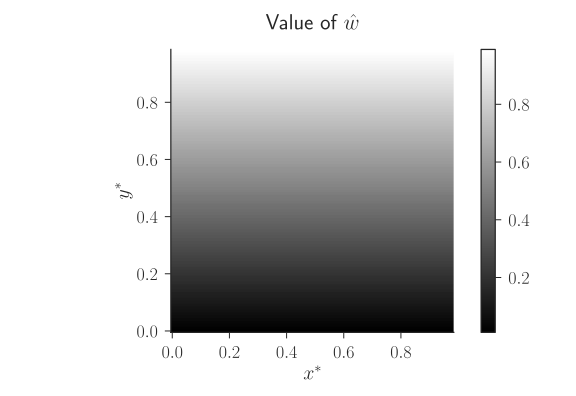
\includegraphics[width=\textwidth]{w-hat-empirical-01-marginal}
\caption{
    Estimates for $\hat{w}$ when computing $(\hat{x}, \hat{y}, \hat{w})$ using basin-hopping \citep{Wales1997} optimizing the classical marginal likelihood \eqref{eq:marginal_likelihood} (rather than a joint optimization procedure).
}
\label{fig:bl-general-marginal}
\end{figure}

\begin{figure}
\centering
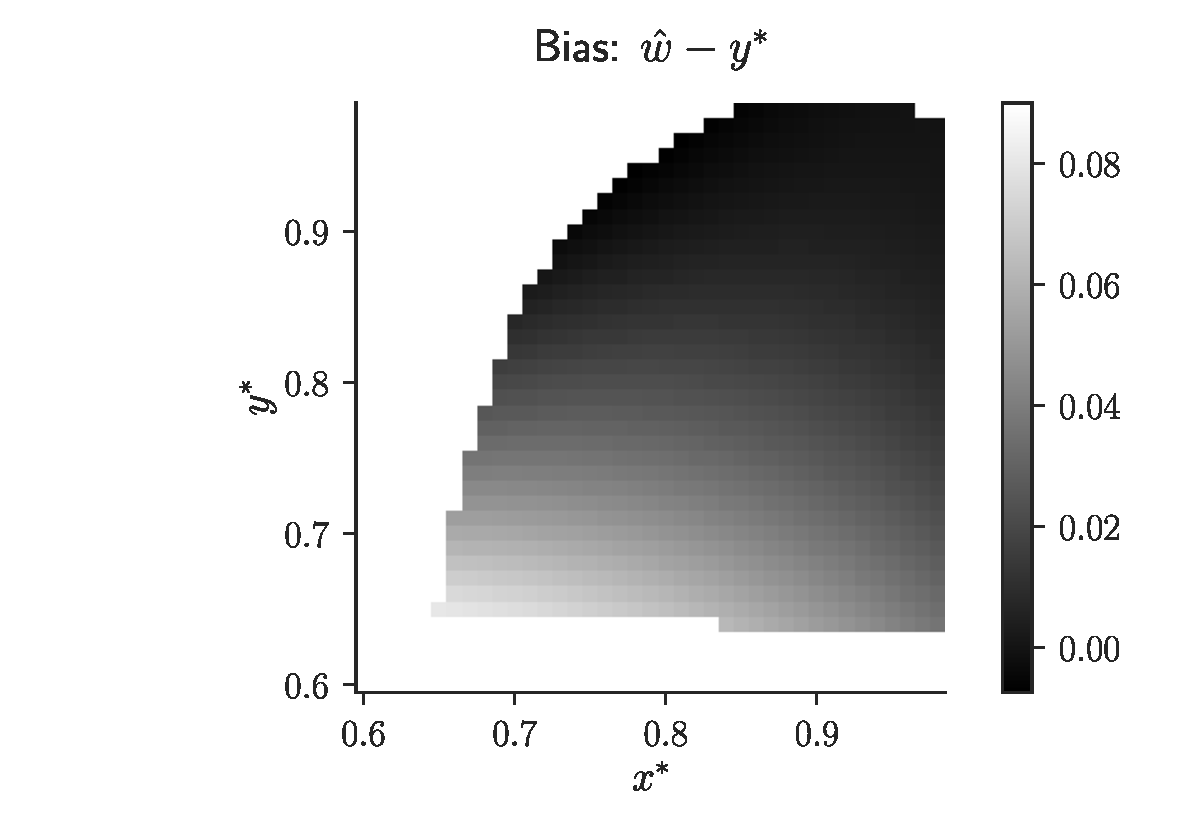
\includegraphics[width=\textwidth]{w-hat-empirical-01-bias}
\caption{
    Estimates for $\hat{w}-y^*$ when computing $(\hat{x}, \hat{y}, \hat{w})$ using basin-hopping \citep{Wales1997} optimizing \eqref{eq:profile_likelihood}.
    Plot focuses on $0.6 < x^*, y^* < 1$ where $\hat{w}$ is estimated to be a value different from 1.
    We do not compute the bias for the white region where $\hat{w}=1$ to preserve a useful scale for the rest of the plot.
}
\label{fig:bl-general-bias}
\end{figure}



\end{document}
